% !TeX spellcheck = hu_HU
% !TeX encoding = UTF-8

% TODO Change language to en_GB (recommended) or en_US for English documents
\documentclass[11pt,a4paper,oneside]{report}             % Single-side
%\documentclass[11pt,a4paper,twoside,openright]{report}  % Duplex

% thanks to http://tex.stackexchange.com/a/47579/71109
\usepackage{ifxetex}
\usepackage{ifluatex}
\newif\ifxetexorluatex % a new conditional starts as false
\ifnum 0\ifxetex 1\fi\ifluatex 1\fi>0
   \xetexorluatextrue
\fi

\ifxetexorluatex
  \usepackage{fontspec}
\else
  \usepackage[T1]{fontenc}
  \usepackage[utf8]{inputenc}
  \usepackage[lighttt]{lmodern}
\fi

\usepackage[english,magyar]{babel} % Alapértelmezés szerint utoljára definiált nyelv lesz aktív, de később külön beállítjuk az aktív nyelvet.

%\usepackage{cmap}
\usepackage{amsfonts,amsmath,amssymb} % Mathematical symbols.
%\usepackage[ruled,boxed,resetcount,linesnumbered]{algorithm2e} % For pseudocodes. % beware: this is not compatible with LuaLaTeX, see http://tex.stackexchange.com/questions/34814/lualatex-and-algorithm2e
\usepackage{booktabs} % For publication quality tables for LaTeX
\usepackage{graphicx}
\usepackage{grffile}

%\usepackage{fancyhdr}
%\usepackage{lastpage}

\usepackage{anysize}
%\usepackage{sectsty}
\usepackage{setspace} % For setting line spacing

\usepackage[unicode]{hyperref} % For hyperlinks in the generated document.
\usepackage{xcolor}
\usepackage{listings} % For source code snippets.

\usepackage[amsmath,thmmarks]{ntheorem} % Theorem-like environments.

\usepackage[hang]{caption}

\newcommand{\todo}{\textcolor{red}{TODO !}}
\newcommand{\laci}{\textcolor{red}{TODO !}}

\newcommand{\new}{\textcolor{green}{ÚJDONSÁG!!}}


\singlespacing

\newcommand{\selecthungarian}{
	\selectlanguage{magyar}
	\setlength{\parindent}{2em}
	\setlength{\parskip}{0em}
	\frenchspacing	
}

\newcommand{\selectenglish}{
	\selectlanguage{english}
	\setlength{\parindent}{0em}
	\setlength{\parskip}{0.5em}
	\nonfrenchspacing
	\renewcommand{\figureautorefname}{Figure}
	\renewcommand{\tableautorefname}{Table}
	\renewcommand{\partautorefname}{Part}
	\renewcommand{\chapterautorefname}{Chapter}
	\renewcommand{\sectionautorefname}{Section}
	\renewcommand{\subsectionautorefname}{Section}
	\renewcommand{\subsubsectionautorefname}{Section}
}


%TODO Set the main variables
\newcommand{\vikszerzoVezeteknev}{Bulla}
\newcommand{\vikszerzoKeresztnev}{Ádám}

\newcommand{\vikkonzulensAMegszolitas}{dr.~}
\newcommand{\vikkonzulensAVezeteknev}{Czap}
\newcommand{\vikkonzulensAKeresztnev}{László}

\newcommand{\vikkonzulensBMegszolitas}{dr.~}
\newcommand{\vikkonzulensBVezeteknev}{Buttyán}
\newcommand{\vikkonzulensBKeresztnev}{Levente}

\newcommand{\vikkonzulensCMegszolitas}{}
\newcommand{\vikkonzulensCVezeteknev}{}
\newcommand{\vikkonzulensCKeresztnev}{}

\newcommand{\vikcim}{Identitás információk kezelése biztonsági események kiértékelésében} % Cím
\newcommand{\viktanszek}{\bmehit} % Tanszék
\newcommand{\vikdoktipus}{\msc} % Dokumentum típusa (\bsc, \msc)

%--------------------------------------------------------------------------------------
% TDK-specifikus változók
%--------------------------------------------------------------------------------------
\newcommand{\tdkszerzoB}{Második Szerző} % Második szerző neve; hagyd üresen, ha egyedül í­rtad a TDK-t.
\newcommand{\tdkev}{2014} % A dolgozat írásának éve (pl. "2014") (Ez OTDK-nál eltérhet az aktuális évtől.)

% További adatok az OTDK címlaphoz (BME-s TDK-hoz nem kell kitölteni)
\newcommand{\tdkevfolyamA}{IV} % Első szerző évfolyama, római számmal (pl. IV).
\newcommand{\tdkevfolyamB}{III} % Második szerző évfolyama, római számmal (pl. III).
\newcommand{\tdkkonzulensbeosztasA}{egyetemi tanár} % Első konzulens beosztása (pl. egyetemi docens)
\newcommand{\tdkkonzulensbeosztasB}{doktorandusz} % Második konzulens beosztása (pl. egyetemi docens)

\newcommand{\szerzoMeta}{\vikszerzoVezeteknev{} \vikszerzoKeresztnev} % egy szerző esetén
%\newcommand{\szerzoMeta}{\vikszerzoVezeteknev{} \vikszerzoKeresztnev, \tdkszerzoB} % két szerző esetén

%TODO Language configuration -- choose one
% Beállítások magyar nyelvű dolgozathoz
%--------------------------------------------------------------------------------------
% Elnevezések
%--------------------------------------------------------------------------------------
\newcommand{\bme}{Budapesti Műszaki és Gazdaságtudományi Egyetem}
\newcommand{\vik}{Villamosmérnöki és Informatikai Kar}

\newcommand{\bmehit}{Hálózati rendszerek és szolgáltatások Tanszék}

\newcommand{\keszitette}{Készítette}
\newcommand{\konzulens}{Konzulens}

\newcommand{\bsc}{Szakdolgozat}
\newcommand{\msc}{Diplomaterv}
\newcommand{\bsconlab}{BSc Önálló laboratórium}
\newcommand{\msconlabi}{MSc Önálló laboratórium 1.}
\newcommand{\msconlabii}{MSc Önálló laboratórium 2.}

\newcommand{\pelda}{Példa}
\newcommand{\definicio}{Definíció}
\newcommand{\tetel}{Tétel}

\newcommand{\bevezetes}{Bevezetés}
\newcommand{\koszonetnyilvanitas}{Köszönetnyilvánítás}
\newcommand{\abrakjegyzeke}{Ábrák jegyzéke}
\newcommand{\tablazatokjegyzeke}{Táblázatok jegyzéke}
\newcommand{\irodalomjegyzek}{Irodalomjegyzék}
\newcommand{\fuggelek}{Függelék}

\newcommand{\szerzo}{\vikszerzoVezeteknev{} \vikszerzoKeresztnev}
\newcommand{\vikkonzulensA}{\vikkonzulensAMegszolitas\vikkonzulensAVezeteknev{} \vikkonzulensAKeresztnev}
\newcommand{\vikkonzulensB}{\vikkonzulensBMegszolitas\vikkonzulensBVezeteknev{} \vikkonzulensBKeresztnev}
\newcommand{\vikkonzulensC}{\vikkonzulensCMegszolitas\vikkonzulensCVezeteknev{} \vikkonzulensCKeresztnev}

\newcommand{\selectthesislanguage}{\selecthungarian}

\bibliographystyle{huplain}

\def\lstlistingname{lista}

\newcommand{\appendixnumber}{6}  % a fofejezet-szamlalo az angol ABC 6. betuje (F) lesz

% Settings for English documents
%%--------------------------------------------------------------------------------------
% Elnevezések
%--------------------------------------------------------------------------------------
\newcommand{\bme}{Budapest University of Technology and Economics}
\newcommand{\vik}{Faculty of Electrical Engineering and Informatics}

\newcommand{\bmemit}{Department of Measurement and Information Systems}

\newcommand{\keszitette}{Author}
\newcommand{\konzulens}{Advisor}

\newcommand{\bsc}{Bachelor's Thesis}
\newcommand{\msc}{Master's Thesis}
\newcommand{\bsconlab}{BSc Project Laboratory}
\newcommand{\msconlabi}{MSc Project Laboratory 1}
\newcommand{\msconlabii}{MSc Project Laboratory 2}

\newcommand{\pelda}{Example}
\newcommand{\definicio}{Definition}
\newcommand{\tetel}{Theorem}

\newcommand{\bevezetes}{Introduction}
\newcommand{\koszonetnyilvanitas}{Acknowledgements}
\newcommand{\abrakjegyzeke}{List of Figures}
\newcommand{\tablazatokjegyzeke}{List of Tables}
\newcommand{\irodalomjegyzek}{Bibliography}
\newcommand{\fuggelek}{Appendix}

\newcommand{\szerzo}{\vikszerzoKeresztnev{} \vikszerzoVezeteknev}
\newcommand{\vikkonzulensA}{\vikkonzulensAMegszolitas\vikkonzulensAKeresztnev{} \vikkonzulensAVezeteknev}
\newcommand{\vikkonzulensB}{\vikkonzulensBMegszolitas\vikkonzulensBKeresztnev{} \vikkonzulensBVezeteknev}
\newcommand{\vikkonzulensC}{\vikkonzulensCMegszolitas\vikkonzulensCKeresztnev{} \vikkonzulensCVezeteknev}

\newcommand{\selectthesislanguage}{\selectenglish}

\bibliographystyle{plain}

\newcommand{\ie}{i.e.\@\xspace}
\newcommand{\Ie}{I.e.\@\xspace}
\newcommand{\eg}{e.g.\@\xspace}
\newcommand{\Eg}{E.g.\@\xspace}
\newcommand{\etal}{et al.\@\xspace}
\newcommand{\etc}{etc.\@\xspace}
\newcommand{\vs}{vs.\@\xspace}
\newcommand{\viz}{viz.\@\xspace} % videlicet
\newcommand{\cf}{cf.\@\xspace} % confer
\newcommand{\Cf}{Cf.\@\xspace}
\newcommand{\wrt}{w.r.t.\@\xspace} % with respect to

\newcommand{\appendixnumber}{1}  % a fofejezet-szamlalo az angol ABC 1. betuje (A) lesz


%--------------------------------------------------------------------------------------
% Page layout setup
%--------------------------------------------------------------------------------------
% we need to redefine the pagestyle plain
% another possibility is to use the body of this command without \fancypagestyle
% and use \pagestyle{fancy} but in that case the special pages
% (like the ToC, the References, and the Chapter pages)remain in plane style

\pagestyle{plain}
\marginsize{35mm}{25mm}{15mm}{15mm}

\setcounter{secnumdepth}{0}
%\sectionfont{\large\upshape\bfseries}
\setcounter{secnumdepth}{2}

\sloppy % Margón túllógó sorok tiltása.
\widowpenalty=10000 \clubpenalty=10000 %A fattyú- és árvasorok elkerülése
\def\hyph{-\penalty0\hskip0pt\relax} % Kötőjeles szavak elválasztásának engedélyezése


%--------------------------------------------------------------------------------------
% Setup hyperref package
%--------------------------------------------------------------------------------------
\hypersetup{
    % bookmarks=true,            % show bookmarks bar?
    unicode=true,              % non-Latin characters in Acrobat's bookmarks
    pdftitle={\vikcim},        % title
    pdfauthor={\szerzoMeta},    % author
    pdfsubject={\vikdoktipus}, % subject of the document
    pdfcreator={\szerzoMeta},   % creator of the document
    pdfproducer={},    % producer of the document
    pdfkeywords={},    % list of keywords (separate then by comma)
    pdfnewwindow=true,         % links in new window
    colorlinks=true,           % false: boxed links; true: colored links
    linkcolor=black,           % color of internal links
    citecolor=black,           % color of links to bibliography
    filecolor=black,           % color of file links
    urlcolor=black             % color of external links
}


%--------------------------------------------------------------------------------------
% Set up listings
%--------------------------------------------------------------------------------------
\definecolor{lightgray}{rgb}{0.95,0.95,0.95}
\lstset{
	basicstyle=\scriptsize\ttfamily, % print whole listing small
	keywordstyle=\color{black}\bfseries, % bold black keywords
	identifierstyle=, % nothing happens
	% default behavior: comments in italic, to change use
	% commentstyle=\color{green}, % for e.g. green comments
	stringstyle=\scriptsize,
	showstringspaces=false, % no special string spaces
	aboveskip=3pt,
	belowskip=3pt,
	backgroundcolor=\color{lightgray},
	columns=flexible,
	keepspaces=true,
	escapeinside={(*@}{@*)},
	captionpos=b,
	breaklines=true,
	frame=single,
	float=!ht,
	tabsize=2,
	literate=*
		{á}{{\'a}}1	{é}{{\'e}}1	{í}{{\'i}}1	{ó}{{\'o}}1	{ö}{{\"o}}1	{ő}{{\H{o}}}1	{ú}{{\'u}}1	{ü}{{\"u}}1	{ű}{{\H{u}}}1
		{Á}{{\'A}}1	{É}{{\'E}}1	{Í}{{\'I}}1	{Ó}{{\'O}}1	{Ö}{{\"O}}1	{Ő}{{\H{O}}}1	{Ú}{{\'U}}1	{Ü}{{\"U}}1	{Ű}{{\H{U}}}1
}


%--------------------------------------------------------------------------------------
% Set up theorem-like environments
%--------------------------------------------------------------------------------------
% Using ntheorem package -- see http://www.math.washington.edu/tex-archive/macros/latex/contrib/ntheorem/ntheorem.pdf

\theoremstyle{plain}
\theoremseparator{.}
\newtheorem{example}{\pelda}

%\theoremseparator{.}
%\theoremprework{\bigskip\hrule\medskip}
%\theorempostwork{\hrule\bigskip}
%\theorembodyfont{\upshape}
%\theoremsymbol{{\large \ensuremath{\centerdot}}}
%\newtheorem{definition}{\definicio}

%\theoremseparator{.}
%\theoremprework{\bigskip\hrule\medskip}
%\theorempostwork{\hrule\bigskip}
%\newtheorem{theorem}{\tetel}


%--------------------------------------------------------------------------------------
% Some new commands and declarations
%--------------------------------------------------------------------------------------
\newcommand{\code}[1]{{\upshape\ttfamily\scriptsize\indent #1}}
\newcommand{\doi}[1]{DOI: \href{http://dx.doi.org/\detokenize{#1}}{\raggedright{\texttt{\detokenize{#1}}}}} % A hivatkozások közt így könnyebb DOI-t megadni.

\DeclareMathOperator*{\argmax}{arg\,max}
%\DeclareMathOperator*[1]{\floor}{arg\,max}
\DeclareMathOperator{\sign}{sgn}
\DeclareMathOperator{\rot}{rot}


%--------------------------------------------------------------------------------------
% Setup captions
%--------------------------------------------------------------------------------------
\captionsetup[figure]{
	width=.75\textwidth,
	aboveskip=10pt}

\renewcommand{\captionlabelfont}{\bf}
%\renewcommand{\captionfont}{\footnotesize\it}

%--------------------------------------------------------------------------------------
% Hyphenation exceptions
%--------------------------------------------------------------------------------------
\hyphenation{Shakes-peare Mar-seilles ár-víz-tű-rő tü-kör-fú-ró-gép}


\author{\vikszerzo}
\title{\viktitle}

%--------------------------------------------------------------------------------------
% Table of contents and the main text
%--------------------------------------------------------------------------------------
\begin{document}

%TODO These define guidelines -- remove these
%~~~~~~~~~~~~~~~~~~~~~~~~~~~~~~~~~~~~~~~~~~~~~~~~~~~~~~~~~~~~~~~~~~~~~~~~~~~~~~~~~~~~~~
%\pagenumbering{gobble}
\selecthungarian
%--------------------------------------------------------------------------------------
% Rovid formai es tartalmi tajekoztato
%--------------------------------------------------------------------------------------

\footnotesize
\begin{center}
\large
\textbf{\Large Általános információk, a diplomaterv szerkezete}\\
\end{center}

A diplomaterv szerkezete a BME Villamosmérnöki és Informatikai Karán:
\begin{enumerate}
\item	Diplomaterv feladatkiírás
\item	Címoldal
\item	Tartalomjegyzék
\item	A diplomatervező nyilatkozata az önálló munkáról és az elektronikus adatok kezeléséről
\item	Tartalmi összefoglaló magyarul és angolul
\item	Bevezetés: a feladat értelmezése, a tervezés célja, a feladat indokoltsága, a diplomaterv felépítésének rövid összefoglalása
\item	A feladatkiírás pontosítása és részletes elemzése
\item	Előzmények (irodalomkutatás, hasonló alkotások), az ezekből levonható következtetések
\item	A tervezés részletes leírása, a döntési lehetőségek értékelése és a választott megoldások indoklása
\item	A megtervezett műszaki alkotás értékelése, kritikai elemzése, továbbfejlesztési lehetőségek
\item	Esetleges köszönetnyilvánítások
\item	Részletes és pontos irodalomjegyzék
\item	Függelék(ek)
\end{enumerate}

Felhasználható a következő oldaltól kezdődő \LaTeX diplomatervsablon dokumentum tartalma. 

A diplomaterv szabványos méretű A4-es lapokra kerüljön. Az oldalak tükörmargóval készüljenek (mindenhol 2,5~cm, baloldalon 1~cm-es kötéssel). Az alapértelmezett betűkészlet a 12 pontos Times New Roman, másfeles sorközzel, de ettől kismértékben el lehet térni, ill. más betűtípus használata is megengedett.

Minden oldalon -- az első négy szerkezeti elem kivételével -- szerepelnie kell az oldalszámnak.

A fejezeteket decimális beosztással kell ellátni. Az ábrákat a megfelelő helyre be kell illeszteni, fejezetenként decimális számmal és kifejező címmel kell ellátni. A fejezeteket decimális aláosztással számozzuk, maximálisan 3 aláosztás mélységben (pl. 2.3.4.1.). Az ábrákat, táblázatokat és képleteket célszerű fejezetenként külön számozni (pl. 2.4. ábra, 4.2. táblázat vagy képletnél (3.2)). A fejezetcímeket igazítsuk balra, a normál szövegnél viszont használjunk sorkiegyenlítést. Az ábrákat, táblázatokat és a hozzájuk tartozó címet igazítsuk középre. A cím a jelölt rész alatt helyezkedjen el.

A képeket lehetőleg rajzoló programmal készítsék el, az egyenleteket egyenlet-szerkesztő segítségével írják le (A \LaTeX~ehhez kézenfekvő megoldásokat nyújt).

Az irodalomjegyzék szövegközi hivatkozása történhet sorszámozva (ez a preferált megoldás) vagy a Harvard-rendszerben (a szerző és az évszám megadásával). A teljes lista névsor szerinti sorrendben a szöveg végén szerepeljen (sorszámozott irodalmi hivatkozások esetén hivatkozási sorrendben). A szakirodalmi források címeit azonban mindig az eredeti nyelven kell megadni, esetleg zárójelben a fordítással. A listában szereplő valamennyi publikációra hivatkozni kell a szövegben (a \LaTeX-sablon a Bib\TeX~segítségével mindezt automatikusan kezeli). Minden publikáció a szerzők után a következő adatok szerepelnek: folyóirat cikkeknél a pontos cím, a folyóirat címe, évfolyam, szám, oldalszám tól-ig. A folyóiratok címét csak akkor rövidítsük, ha azok nagyon közismertek vagy nagyon hosszúak. Internetes hivatkozások megadásakor fontos, hogy az elérési út előtt megadjuk az oldal tulajdonosát és tartalmát (mivel a link egy idő után akár elérhetetlenné is válhat), valamint az elérés időpontját.

\vspace{5mm}
Fontos:
\begin{itemize}
	\item A szakdolgozatkészítő / diplomatervező nyilatkozata (a jelen sablonban szereplő szövegtartalommal) kötelező előírás, Karunkon ennek hiányában a szakdolgozat/diplomaterv nem bírálható és nem védhető!
	\item Mind a dolgozat, mind a melléklet maximálisan 15~MB méretű lehet!
\end{itemize}

\vspace{5mm}
\begin{center}
Jó munkát, sikeres szakdolgozatkészítést, ill. diplomatervezést kívánunk!
\end{center}

\normalsize
\selectthesislanguage

%\pagenumbering{gobble}
%--------------------------------------------------------------------------------------
% Feladatkiiras (a tanszeken atveheto, kinyomtatott valtozat)
%--------------------------------------------------------------------------------------
\clearpage
\begin{center}
\large
\textbf{FELADATKIÍRÁS}\\
\end{center}

A feladatkiírást a tanszéki adminisztrációban lehet átvenni, és a leadott munkába eredeti, tanszéki pecséttel ellátott és a tanszékvezető által aláírt lapot kell belefűzni (ezen oldal \emph{helyett}, ez az oldal csak útmutatás). Az elektronikusan feltöltött dolgozatban már nem kell beleszerkeszteni ezt a feladatkiírást.


\selecthungarian

%TODO Titlepage -- choose one from below
%~~~~~~~~~~~~~~~~~~~~~~~~~~~~~~~~~~~~~~~~~~~~~~~~~~~~~~~~~~~~~~~~~~~~~~~~~~~~~~~~~~~~~~
\hypersetup{pageanchor=false}
%--------------------------------------------------------------------------------------
%	The title page
%--------------------------------------------------------------------------------------
\begin{titlepage}
\begin{center}

\includegraphics[width=60mm,keepaspectratio]{figures/bme_logo.pdf}\\
\vspace{0.3cm}
\textbf{\bme}\\
\textmd{\vik}\\
\textmd{\viktanszek}\\[5cm]

\vspace{0.4cm}
{\huge \bfseries \vikcim}\\[0.8cm]
\vspace{0.5cm}
\textsc{\Large \vikdoktipus}\\[4cm]

{
	\renewcommand{\arraystretch}{0.85}
	\begin{tabular}{cc}
	 \makebox[7cm]{\emph{\keszitette}} & \makebox[7cm]{\emph{\konzulens}} \\ \noalign{\smallskip}
	 \makebox[7cm]{\szerzo} & \makebox[7cm]{\vikkonzulensA} \\
	  & \makebox[7cm]{\vikkonzulensB} \\
	  & \makebox[7cm]{\vikkonzulensC} \\
	\end{tabular}
}

\vfill
{\large \today}
\end{center}
\end{titlepage}
\hypersetup{pageanchor=false}

		   % Szakdolgozat/Diplomaterv címlap
%%% TDK címlap
\begin{titlepage}
  \begin{center}  
  
\includegraphics[width=7cm]{./figures/bme_logo.pdf}
  \vspace{0.3cm}
  
  \bme \\
  \vik \\
  \viktanszek \\
  \vspace{5cm}
  
  \huge {\vikcim}
  \vspace{1.5cm}
  
  \large {\textbf{\vikdoktipus}}
  \vfill
    
  {\Large 
  	\keszitette: \\ \vspace{0.3cm}
  	\szerzo \\
	\tdkszerzoB \\
  	\vspace{1.5cm}
  	\konzulens: \\ \vspace{0.3cm}
  	\vikkonzulensA \\
  	\vikkonzulensB \\
  }
  
  \vspace{2cm}
  \large {\tdkev}
 \end{center}
\end{titlepage}
%% Címlap vége	% TDK címlap
%%% OTDK külső címlap
\begin{titlepage}
  	$\;$ 
	\vspace{5cm}
	
	\begin{center}
	\Huge
	\textbf{TDK-dolgozat}\let\thefootnote\relax\footnote{A dolgozat bemutatását a XXXXXXXXX  ``Lorem ipsum dolor sit amet'' című program támogatta.}
	\end{center}
	
	\vspace{13cm}
	
	\Large
	\hspace{8cm} \szerzo
	
	\hspace{8cm} \tdkszerzoB
	
	\hspace{8cm} \tdkev.
\end{titlepage}

\newpage
\thispagestyle{empty}


%% OTDK belső címlap
\begin{titlepage}
  \begin{center}  
  
\includegraphics[width=7cm]{./figures/bme_logo.pdf}
  \vspace{0.3cm}
  
  \bme \\
  \vik \\
  \viktanszek \\
  \vspace{3.5cm}
  
  \huge {\vikcim}
  \vspace{1.5cm}
  
  \large {\textbf{\vikdoktipus}}
  \vfill
    
  {\Large 
  	{\large \keszitette:} \\ \vspace{0.2cm}
  	\szerzo \\ \tdkevfolyamA. évfolyam \\
	\vspace{0.5cm}
	\tdkszerzoB \\ \tdkevfolyamB. évfolyam \\
  	\vspace{1.5cm}
  	{\large \konzulens:} \\ \vspace{0.2cm}
  	\vikkonzulensA,\\ \tdkkonzulensbeosztasA \\
  	\vspace{0.5cm}
  	\vikkonzulensB,\\ \tdkkonzulensbeosztasB \\
  }
  
  \vspace{2cm}
  \large {\tdkev.}
  
 \end{center}
\end{titlepage}   % OTDK címlap


% Table of Contents
%~~~~~~~~~~~~~~~~~~~~~~~~~~~~~~~~~~~~~~~~~~~~~~~~~~~~~~~~~~~~~~~~~~~~~~~~~~~~~~~~~~~~~~
\tableofcontents\vfill


% Declaration and Abstract
%~~~~~~~~~~~~~~~~~~~~~~~~~~~~~~~~~~~~~~~~~~~~~~~~~~~~~~~~~~~~~~~~~~~~~~~~~~~~~~~~~~~~~~
\selectlanguage{magyar}
\pagenumbering{gobble}
%--------------------------------------------------------------------------------------
% Nyilatkozat
%--------------------------------------------------------------------------------------
\begin{center}
\large
\textbf{HALLGATÓI NYILATKOZAT}\\
\end{center}

Alulírott \emph{\vikszerzoVezeteknev{} \vikszerzoKeresztnev}, szigorló hallgató kijelentem, hogy ezt a diplomatervet meg nem engedett segítség nélkül, saját magam készítettem, csak a megadott forrásokat (szakirodalom, eszközök stb.) használtam fel. Minden olyan részt, melyet szó szerint, vagy azonos értelemben, de átfogalmazva más forrásból átvettem, egyértelműen, a forrás megadásával megjelöltem.

Hozzájárulok, hogy a jelen munkám alapadatait (szerző(k), cím, angol és magyar nyelvű tartalmi kivonat, készítés éve, konzulens(ek) neve) a BME VIK nyilvánosan hozzáférhető elektronikus formában, a munka teljes szövegét pedig az egyetem belső hálózatán keresztül (vagy autentikált felhasználók számára) közzétegye. Kijelentem, hogy a benyújtott munka és annak elektronikus verziója megegyezik. Dékáni engedéllyel titkosított diplomatervek esetén a dolgozat szövege csak 3 év eltelte után válik hozzáférhetővé.

\begin{flushleft}
\vspace*{1cm}
Budapest, \today
\end{flushleft}

\begin{flushright}
 \vspace*{1cm}
 \makebox[7cm]{\rule{6cm}{.4pt}}\\
 \makebox[7cm]{\emph{\vikszerzoVezeteknev{} \vikszerzoKeresztnev}}\\
 \makebox[7cm]{hallgató}
\end{flushright}
\thispagestyle{empty}

\vfill
\clearpage
\thispagestyle{empty} % an empty page

\selectthesislanguage
 %TODO Hallgatói nyilatkozat -- TDK és OTDK esetén törlendő!
%\pagenumbering{roman}
\setcounter{page}{1}

\selecthungarian

%----------------------------------------------------------------------------
% Abstract in Hungarian
%----------------------------------------------------------------------------
\chapter*{Kivonat}\addcontentsline{toc}{chapter}{Kivonat}

Az informatika fejlődésével és terjedésével egyre fontosabb terület lesz az informatikai biztonságtechnika ami számos feladatot foglal magába. Jelen dolgozat ezen belül kettő területre, a biztonsági incidensek és események kezelésére, valamint a felhasználó és hozzáférés menedzsmentre fókuszál. Mindkét területen elérhetők elérhetők ipari megoldások, mint például az IBM QRadar, és Identity Manager terméke, azonban a két terület jellemzően csak lazán kapcsolódik egymással, szorosabb integrációra technikai megoldás sem állt rendelkezésre korábban.

A dolgozat célja egy ilyen integráció elkészítése és bemutatása a fent említett két termék használatával. A cél az ISIM-ből a felhasználói, és a hozzájuk kötődő folyamat információk összegyűjtése, transzformálása, majd prezentálása a QRadar számára a szabályrendszerében való felhasználásra. Ezek segítségével az egyes események új kontextusban, új információk birtokában értékelhetők ki, ami eddig nem kezelt biztonsági incidensek észlelését teszi lehetővé, ezzel teljesebbé és pontosabbá téve a biztonsági monitorozást.


A dolgozat az adatok elérhetővé tételére két megoldást mutat be: egy JAVA EE alapú webalkalmazást, és egy IBM adatintegrációs eszköz alapú megoldást. A két rendszer közti további integrációra az említett mellett egy saját megoldást is készítettem, ami olyan, a felhasználói folyamatokkal kapcsolatos eseményeket továbbít a QRadar számára,  amik eddig a SIEM számára láthatatlonok voltak.


\vfill
\selectenglish


%----------------------------------------------------------------------------
% Abstract in English
%----------------------------------------------------------------------------
\chapter*{Abstract}\addcontentsline{toc}{chapter}{Abstract}

With the continous advancement of computers and technology, IT Security is becoming an increasingly important field of study, which includes a multitude of tasks. This thesis focuses on two fields of IT security: security information and event management, and identity and access management. Both of these fields have industry solutions available for years, like IBM QRadar, and IBM Security Identity Manager, but the two areas are typically loosely connected, for a more tight integration there was no technical solution available yet.

The aim of this thesis project is to implement and present a solution for this problem, using the aforementioned two products. The goal is the collection, transformation, and presentation of user identity and access information, including the processes managing these from ISIM to QRadar. With this data, the security events handled by QRadar can be evaluatied in a new context, detecting previously unhandled incidents making security monitoring more complete and accurate.

This thesis presents two solutions for this integration: a Java EE based web application, and a custom solution, using an IBM data integration framework. For further integration between the two products, I've also developed a different integration solution, which generates security events for QRadar, from previously unseen events about processes managing user data and access information.


\vfill
\selectthesislanguage

\newcounter{romanPage}
\setcounter{romanPage}{\value{page}}
\stepcounter{romanPage}    %TODO Összefoglaló -- TDK és OTDK esetén nem kötelező


% The main part of the thesis
%~~~~~~~~~~~~~~~~~~~~~~~~~~~~~~~~~~~~~~~~~~~~~~~~~~~~~~~~~~~~~~~~~~~~~~~~~~~~~~~~~~~~~~
\pagenumbering{arabic}

%TODO import your own content
%----------------------------------------------------------------------------
\chapter{\bevezetes}
%----------------------------------------------------------------------------
\label{ch:bev}
\selecthungarian

\section{A dolgozat célja és felépítése }
A modern informatika egyik fontos és feltörekvő területe az IT Security, amely a számítógép ipar fejlődésével egyre nagyobb szerepet kap. Ahogy a gépek számító kapacitása növekszik, egyre könnyebben megoldhatók olyan problémák, amelyek addig lehetetlennek, elfogadható időben kivitelezhetetlennek tűntek. Ez a fejlődés az egész szektort arra készteti, hogy folyamatosan fejlődjön, a meglévő alkalmazásokat, módszereket, algoritmusokat javítsa. Emellett a modern világban egyre nagyobb vállalatok jönnek létre, amelyeknek egyre nagyobb személyzetre van szükségük a működéshez, ami indokolttá teszi egy megfelelően stabil és jól kezelhető informatikai támogató réteg kialakítását. Több ezer, akár több tízezer alkalmazott mellett gyorsan átláthatatlanná válik, hogy kinek milyen eszközökhöz, akár hardveres, akár szoftvereshez van hozzáférése, ezek egyesével való beállítása és karbantartása pedig emberi léptékkel mérve szinte kivitelezhetetlen, és rendkívül költséges a fent említett támogató szoftverek nélkül.

 Jelen dolgozat az IT Security világának számos területéből kettővel foglalkozik, ennek a kettőnek is elsősorban a kapcsolatával. Az egyik terület a Security Information and Event Management (SIEM), ami egy informatikai rendszer biztonsági felügyeletével foglalkozik. A másik terület az Identity management (IdM), ami pedig az alkalmazottak és a hozzájuk tartozó jogosultságok életciklusának menedzselésével foglalkozik. A cél a kettő terület összekapcsolása oly módon, hogy az IdM szoftverben található hasznos, felhasználókkal kapcsolatos adatok elérhetők legyenek a SIEM szoftver számára. Ezek olyan kontextust szolgáltatnak, amely az elemi eseményekből nem következik. Például a SIEM által feldolgozott események jellemzően köthetők egy felhasználónévhez, viszont nem állnak rendelkezésre azok az információk, hogy az adott felhasználónév mely valós személyhez tartozik és az illető esetleg kiléptetés alatt áll-e, a biztonsági házirenddel összhangban van-e egy adott fiók létezése és jogosultsági szintje, vagy hogy mikor és ki hagyta jóvá a felhasználói fiók létrehozását. Mindezen adatok az IdM rendszerből kinyerhetők. Az integráció célja, hogy az IdM rendszerben tárolt releváns adatokkal tudjuk támogatni a SIEM szabályrendszerét.

Egy ilyen integrációval az alábbiak, valamint ehhez hasonló use-case-ek valósíthatók meg:

\begin{itemize}
	\item Inaktív személyekhez tartozó felhasználói fiókok - Ez az információ hasznos lehet egy QRadar szabályhoz például olyan esetben, ha arra vagyunk kíváncsiak, hogy volt-e aktivitás olyan fiókkal, amelynek a tulajdonosa már nem a cég alkalmazottja, és a fióknak meg kellett volna szűnnie.
	
	\item Valós személyhez nem köthető felhasználói fiókok - Ezek az árva fiókok biztonsági kockázatokat jelenthetnek, mert a hozzájuk tartozó műveletekért nincs kit felelősségre vonni. Ezért hasznos lehet egy olyan QRadar szabály, ami kifejezetten az ilyen esetekben jelez.
	
	\item Adott erőforráshoz legitim hozzáféréssel rendelkező személyek - Ez az információ olyan esetben lehet hasznos, ha például egy támadás kiinduló pontjaként sikerül azonosítani egy eszközt. Ezzel lehetséges az olyan felhasználói fiókkal történő aktivitás észlelése, amelyet az IdM szabályrendszerét megkerülve hoztak létre.
\end{itemize}

A diplomatervem keretében fejlesztettem egy integrációs modult, amely egy általános célú adatszinkronizációs eszköz az IdM és a SIEM rendszer között, valamint ennek segítségével megvalósítottam a fent leírt use-case-ekhez szükséges lekérdezéseket és adatszinkronizációt.

A SIEM számára nemcsak a felhasználókkal kapcsolatos adatok, hanem a jogosultságkezeléssel kapcsolatos folyamatok eseményei is relevánsak, amelyeknek szintén az IdM rendszer a forrása. A diplomatervem során megvalósítottam egy olyan eszközt, amely bővíti a SIEM számára látható IdM események körét, ezzel teljesebbé téve az IdM rendszer biztonsági monitorozását.

A dolgozat felépítése a következő:

\begin{itemize}
	\item Az \ref{ch:bev}. fejezet a dolgozat valamint a diplomaterv célját definiálja és járja körbe, rövid bemutatót adva a felhasznált technológiák főbb tulajdonságairól.
	
	\item A \ref{ch:tech}. fejezet a projektben megismert és felhasznált technológiákat mutatja be, kitérve a feladat számára fontos technológiákra.
	
	\item A \ref{ch:imp}. fejezet a konkrét implementációs kérdéseket, valamint az ezekre adott megoldásaimat mutatja be.
	
	\item A \ref{ch:usage}. fejezet az elkészült megoldások telepítését és használatát mutatja be.
	
	\item A \ref{ch:sum}. fejezet egy rövid összefoglaló a féléves munkámról.
	
\end{itemize}

\section{Security Information and Event Management}

A Security Information and Event Management az informatikai rendszer részeinek monitorozásával foglalkozik biztonsági szempontból. Az infrastruktúrában található eszközök által generált eseményekhez hozzáfér a SIEM megoldás, és ez végzi az események feldolgozását és elemzését. A monitorozott rendszerek működésükkel kapcsolatos információkat biztosítanak a SIEM irányába valamilyen formában, általában log sorokként. A SIEM szerver ezeket feldolgozza, és a szabályrendszerének megfelelő eseményekből úgynevezett biztonsági incidenseket hoz létre, akár egyéb forrásokból érkező plusz információk felhasználásával. Ilyen egyéb forrás lehet hálózati forgalom, valamilyen adatbázisból lekért adatok, vagy előre definiált, a szerverre feltöltött adatok. 

Nem triviális feladat a szabályrendszert úgy konfigurálni, hogy a fals pozitív riasztások száma alacsony maradjon, miközben a valós támadásokat hatékonyan detektálja. 

A megvalósítandó integráció a szabályrendszer hatékonyságát kétféleképpen segíti elő. Egyrészt, az IdM-ben redelkezésre álló információk segítségével olyan támadásminták detekciója válik lehetővé, amelyeket enélkül a SIEM nem lenne képes észlelni. Másrészt, a SIEM szabályrendszerét aktuális adatokkal látja el, amely a fals pozitív riasztások számát képes csökkenteni.

Emellett az általam generált és feldolgozott IdM-ből érkező jogosultsági folyamatok eseményein keresztül a SIEM további, fontos incidenseket képes detektálni.

Jelen feladatnak nem célja a SIEM szabályrendszerének részletes kidolgozása, a dolgozat témája az IdM és a SIEM közötti adatszinkronizáció lehetőségének megteremtése.

\section{Identity management}

Az Identity management a fejlődő nagyvállalatok fent említett problémáiból a nagyszámú alkalmazott hozzáféréseinek kezelését és a dolgozók, mint informatikai entitások életciklusának menedzselését oldja meg. Ez magában foglalja az entitások  rendszerezését, csoportokhoz rendelését, valamint a saját és örökölt jogaik érvényre juttatását.

Minden alkalmazotthoz tartozik egy rekord, amely leírja az adott ember személyes adatait és egyéb olyan információkat, amelyek szükségesek az alkalmazott jogosultságainak meghatározásához. Ezt a létrejött entitást beosztja a megadott információk szerint a megfelelő, előre definiált szerepkörökbe, amely alapján az jogokat kap bizonyos eszközök használatára. Ezen eszközök is entitásként vannak felvéve a rendszerbe, oly módon, hogy elérhetők az eszközhöz (akár szoftveres akár hardveres) tartozó információk és menedzselhető a hozzáférés.

A dolgozat célja ezen alkalmazotti és a hozzájuk kapcsolódó életciklus információinak kinyerése és eljuttatása a SIEM rendszer számára, mivel ezek az információk értékesek lehetnek a biztonsági incidensek kiértékelése szempontjából.

\section{A feladat specifikálása}

Jelen dolgozat feladata egy olyan megoldás fejlesztése, mely lehetővé teszi a fent említett technológiák közti integrációt és az adatszinkronizációt. Az integrációt a IBM által kínált IdM (IBM Security Identity Manager - ISIM\footnote{Lásd \ref{subsec:ISIM} \nameref{subsec:ISIM}}) és SIEM (IBM Security QRadar SIEM - QRadar\footnote{Lásd \ref{subsec:qradar} \nameref{subsec:qradar}}) között dolgoztam ki.
 
A végső megoldás két részből áll, egyrészt egy teljesen új funkcionalitást biztosító integrációs modulból, valamint egy már meglévő funkcionalitást bővítő kiegészítésből. Erre a feladatra eddig nem volt automatikus megoldás, ezért ez a projekt ezt a hiányt hivatott betölteni.

A QRadarban már megtalálható egy olyan modul, ami képes az ISIM-ben generált események egy részhalmazának feldolgozására és értelmezésére, de ez csak bizonyos audit események feldolgozására képes. Ezt kibővítendő készítettem egy megoldást, amely az előző funkcionalitást egészíti ki egyéb, eddig nem feldolgozott eseményekkel, amelyek plusz információt hordoznak biztonsági szempontból. A modulhoz használt keretrendszert a TDI \footnote{\label{foot:TDI}Lásd \ref{subsec:TDI} \nameref{subsec:TDI}} nyújtja.

Mindkét integráció megvalósításához a Java alapú technológiát választottuk. A döntést indokolja, hogy jól illeszkedik a tipikus nagyvállalati környezethez, az IBM kiterjedt tapasztalattal és eszközkészlettel rendelkezik ezen a téren, valamint ez az ISIM technológiája és programozói interfésze is.

Az integráció megvalósításának első lépése egy Java API fejlesztése a QRadar-hoz. A QRadar egy technológiafüggetlen REST API-val rendelkezik. Ahhoz, hogy Java alkalmazásból az API számunkra fontos része használható legyen, egy Java Wrapper library-t fejlesztettem, amely Java metódusok formájában teszi lehetővé a QRadar API használatát. Ez a wrapper egy általános megoldást ad a QRadarba feltöltött adatok (lsd. \ref{lbl:reference_data}) lekérésére és módosítására, így egy később felmerülő projektben is hasznos lehet.

Az integráció megvalósítására két architektúrát is kidolgoztunk, amelyeket a következő két alfejezetben ismertetek.

\subsection{Integráció TDI segítségével}

A Tivoli Directory Integrator (TDI \footnote{\label{foot:TDI}Lásd \ref{subsec:TDI} \nameref{subsec:TDI}}) egy gyakran használt, általános célú integrációs eszköz. 
A TDI segítségével különböző adatforrásokat, amelyek más-más protokollon keresztül érhetők el, és más-más formátumban és struktúrában tárolják az adatokat, egy egységes ú.n.~Connector interfészen keresztül érhetjük el. Az adattranszformációs feladatokat ú.n.~assembly line formájában valósíthatjuk meg a TDI grafikus felületén. Egy assembly line egy műveletsort definiál, amely során felhasználhatjuk a connectorokat adat olvasásra, keresésre, kiírásra, valamint Javascript segítségével tetszőleges adattranszformációt valósíthatunk meg. A megfelelő protokoll és parser kiválasztásáról a használt connector gondoskodik, így az assembly line kompakt módon csak a valódi adattranszformációt definiálja. 

A TDI gyári connector készletét kiegészítettem egy új, saját fejlesztésű connectorral, amely a fent említett wrapper könyvtár segítségével képes reference data-kat feltölteni és lekérni a QRadartól. A hálózati erőforrások hatékony használatának céljából a connector külön akkumulálja a feltöltendő adatokat, és a futása végén, egyben tölti azokat fel. Az általam létrehozott connector egy általános célú TDI connector, így szabadon újra felhasználható nem csak az ISIM-mel való integrációra, hanem tetszőleges TDI assembly line formájában megvalósított integrációs feladatra. 

Ebben a megvalósításban a QRadar és az ISIM közti integrációt TDI assembly line-ok formájában valósítottam meg, melyeket a TDI által biztosított szerver komponens dolgoz fel és futtat. A TDI gyári funkcióit és grafikus interfészét felhasználva az egyes assembly line-ok fejlesztése időtakarékos és költséghatékony. Ennek a megvalósításnak hátránya, hogy a megoldások a TDI-hez kötöttek, valamint a lehetőségeknek határt szabnak a TDI által nyújtott lehetőségek. Egy újabb lekérdezés vagy lekérdezéstípus konfigurálása, ütemezése a TDI fejlesztői felületén történik, így az üzemeltetési feladatok ellátásához a TDI ismerete szükséges.


\begin{figure}[]
	\centering
	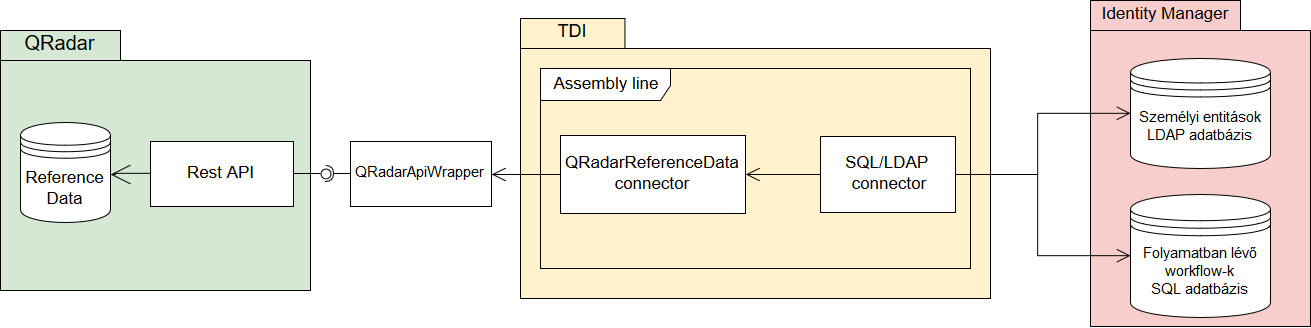
\includegraphics[width=1.0\linewidth]{figures/TDI_architecture.png}
	\caption{Architektúra TDI esetén}
	\label{fig:tdi-architecture}
	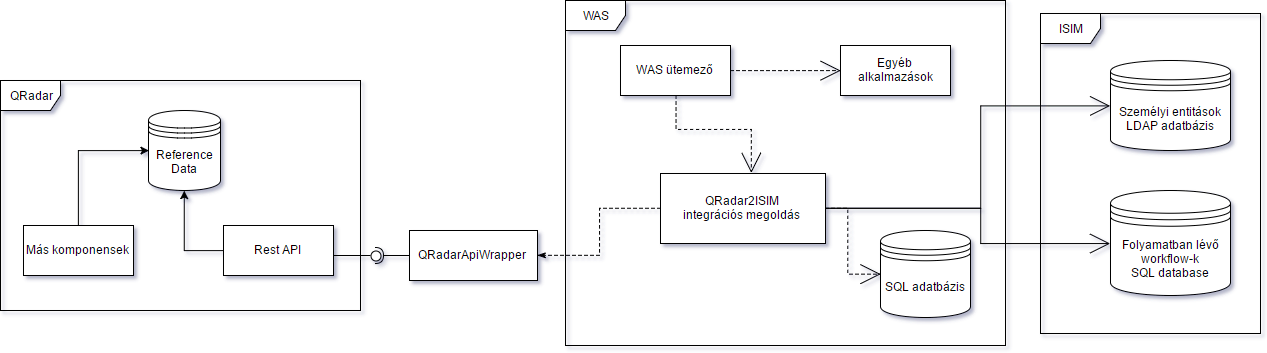
\includegraphics[width=1.0\linewidth]{figures/WAS_architecture.png}
	\caption{Architektúra WAS esetén}
	\label{fig:wasarchitecture}
\end{figure}


\subsection{Integráció webes (WAS) alkalmazás formájában}

Ennél a megoldásnál egy IBM WebSphere Application Server (WAS) környezetre fejlesztett alkalmazást készítettünk egy projekt keretében, amely a QRadarral való kommunikációra felhasználja az általam fejlesztett wrapper-t. Az alkalmazás rendelkezik egy felhasználóbarát webes felülettel, melyen keresztül létrehozhatunk és felkonfigurálhatunk szinkronizációs feladatokat. Az integrációt olyan szinkronizációs feladatok valósítják meg, melyek ütemezett futtatására támogatást biztosít az alkalmazás a WAS által nyújtott lehetőségeken keresztül. A feladatok eltárolják az aktuálisan lekérdezett adatokat egy SQL adatbázisba, valamint karbantartanak egy másik táblát ami mindig a QRadarra aktuálisan sikeresen felszinkronizált adatokat tartja számon. Ezen adatbázisok segítségével számolható egy különbség, ami az elégségesen felküldendő adatokat tartalmazza. Ezzel csökkenthető a QRadar irányába a tranzakciónkénti overhead. Emellett ha az alkalmazás inkonzisztenciát érzékel a lokális állapot és a QRadarban megtalálható adatok között, akkor egy teljes szinkronizációval minden adatot felküld, ezzel egy új, konzisztens állapotba állítva a rendszert.

%Ebben a megvalósításban TDI alapú megoldáshoz képest előny, hogy az integrációs adatokhoz tartozó szinkronizáció pontos implementációja saját fejlesztésű, így hozzáigazítható a pontos igényekhez. 
Ebben a megvalósításban a TDI alapú megoldáshoz képest előny, hogy a WAS egy menedzselt környezetet biztosít a futtatáshoz, így jobban felügyelhetők az egyes feladatok, valamint igény szerint könnyen megvalósítható az elosztott, klaszteren futó, hibatűrő működés is. Előny továbbá, hogy saját grafikus felhasználói felülettel rendelkezik, amelyen az üzemeltetési feladatok könnyen elvégezhetők. Új lekérdezéstípus létrehozása Java fejlesztői ismeretet követel meg, konkrét technológiához kötött (pl.~TDI) tudás nem szükséges. A WAS minden ISIM környezetben elérhető, ezért nem szükséges új komponensek telepítése az modul használatához.

A TDI-t használó megoldással szemben a hátránya, hogy a megoldás ISIM specifikus, más forrásokkal való integrációhoz szükség van a forráskód módosítására.

%----------------------------------------------------------------------------
\chapter{Irodalomkutatás és a felhasznált technológiák}
\label{ch:tech}
%----------------------------------------------------------------------------
\section{A felhasznált technológiák ismertetése}
%----------------------------------------------------------------------------
Mivel a feladat egy specifikus alkalmazás előállítása volt, amely már létező termékek közötti kommunikációt biztosít, ezért ennek jelentős része volt a termékekkel való alapszintű, valamint a felhasznált specifikus funkciókkal és interfészekkel való mélyebb ismerkedés.


\subsection{IBM Security QRadar SIEM}
\label{subsec:qradar}
Az IBM Security QRadar SIEM az IBM security information and event manager rendszere, ami lehetővé teszi hálózatra csatlakoztatott eszközöknek a megfigyelését biztonsági szempontból.\cite{qradardoc} A hálózaton elosztott több ezernyi eszközvégpontból és alkalmazásból származó napló fájl eseményadatait összesíti, és a nyers adatokon azonnali normalizálási és összesítési műveleteket végez. Az eseménynaplók betöltésére számos automatikus módszer áll rendelkezésre, többek közt olyan közismert protokollok mint a SYSLOG, SNMP, FTP, SCP. Az IBM Security QRadar SIEM ugyancsak képes a rendszer sebezhetőségeinek és az esemény- és hálózati adatoknak az összevetésére, ezáltal segítséget nyújt a biztonsági incidensek rangsorolásában. Emellett lehetőség van egyéb adatforrások felvételére a felhasználó által is, amelyek szintén használhatók a fenyegetések és az incidensek detektálásában. Ezek jelentősége elsősorban a dinamikus szabályok létrehozásában játszik nagy szerepet, mivel ezek segítségével egy API-n keresztül karbantarthatók a létrehozott dinamikus szabályok. A szinkronizáció megvalósítására nincs egységes módszer vagy eszköz, ezt minden esetben az adatok jellege és az adatforrás által biztosított interfész határozza meg.

\begin{figure}
	\centering
	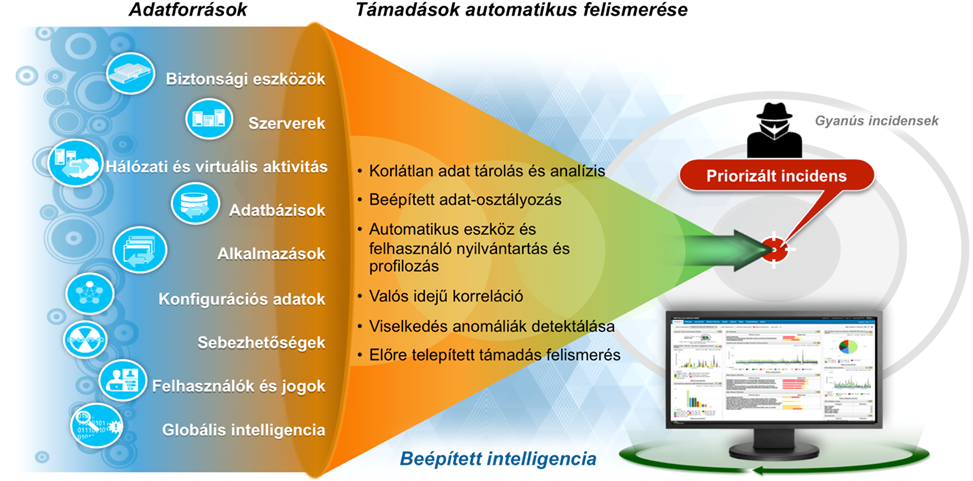
\includegraphics[width=0.9\linewidth]{figures/QRadar_promo.png}
	\caption{QRadar funkciói.}
	\label{fig:qradar-promo}
\end{figure}

Felvehetők a SIEM-be bizonyos sablonok alapján összeállítható szabályok, amelyeket a rule engine kiértékel a beérkező eseményekre. A kiértékelés alapján az eseményeket besorolja a megfelelő csoportokba súlyosságuk és egyéb tulajdonságaik alapján, vagy ha szükséges létrehoz egy új, különálló eseményt. Az incidensek kezelésére külön felület szolgál, illetve különböző interfészeken keresztül értesítést tud küldeni ezekről a rendszer. Ezen túl minden feldolgozott esemény később megtekinthető keresések és szűrések segítségével.

A SIEM által kiértékelt eseményekhez egyéb információkat is rendel a rendszer, olyanokat, mint például a támadás típusa, az esemény leírása, a résztvevő felek adatai, melyeket később is meg lehet tekinteni, valamint segítségükkel és az egyéb környezeti forgalommal együtt egy egész hálózat működése visszajátszható.
%\begin{comment}
%	A plusz információk közé tartozik egy 3 szempontú értékelés is, amely alapján a QRadar számolja az egyes esetek súlyosságát.
%	\begin{itemize}
%	\item Súlyosság (Severity) - a súlyosság jelzi hogy a támadó milyen fenyegetettséget jelent annak függvényében hogy mennyire sebezhető a megcélzott eszköz.
	
%	\item Hitelesség (Credibility) – a hitelesség jelzi az integritását vagy valódiságát egy támadásnak, amelyik érték az eseményt generáló biztonsági eszköztől érkezik. A hitelesség növekedhet, ha a különböző források is jelentik ugyanazt az eseményt.
	
%	\item Relevancia (Relevance) – a relevancia meghatározza azt, hogy a célpont milyen értéket képvisel a hálózaton.
%	\end{itemize}
%\end{comment}
 
\label{lbl:reference_data}
Ezen dokumentum és a feladat szempontjából a legfontosabb része a QRadarnak a dinamikusan feltölthető adathalmazok és azok használata szabályokban. Ezekkel a szabályokkal érhető el, hogy más adatforrásokból (jelen esetben az ISIM-ből) frissen feltöltött információk alapján változzon a kiértékelés, és ha valamilyen adat frissül, akkor naprakész maradjon a szabály által talált incidensek halmaza. A dinamikusan feltölthető adathalmazok (összefoglaló nevükön reference data) elérhetők egy REST API-n keresztül, így könnyen hozzájuk lehet férni és módosítani őket. Négy féle ilyen adathalmaz áll rendelkezésre:

\begin{itemize}
	\item Reference set - Olyan adathalmaz, melyben egyedi értékek sorozata található.
	\item Reference map - Olyan adathalmaz, melyben kulcs-érték párok találhatók, a kulcsok egyediek, és szigorúan szöveges adatok.
	\item Reference map of sets - Olyan adathalmaz, melyben kulcs-halmaz párok találhatók, a kulcsok egyediek, szövegesek, és a halmazban saját csoportjukban egyedi értékek találhatók.
	\item Reference map of maps (tables) - Olyan adathalmaz, melyben kulcs-kulcs-érték triplet összerendelések találhatók.
\end{itemize}

Minden reference data-nak van egy típusa, ami meghatározza hogy az adott halmazban milyen típusú értékek találhatók.

\begin{itemize}
	\item ALN - Alfanumerikus karakterek
	\item ALNIC - Alfanumerikus karakterek, figyelmen kívül hagyva a kis- és nagybetű közti különbséget 
	\item IP - IP címek
	\item NUM - Numerikus karakterek
	\item PORT - Port számok
	\item DATE - Dátumok, miliszekundomokban 1970.01.01 óta
\end{itemize}

Emellett a reference data-ban található adatoknak lehet egy time-to-live (TTL -- elévülési idő) értéke is, ami meghatározza, hogy mennyi idő elteltével törlendő az adott adat. Ennek 3 típusa lehet: 
\begin{itemize}
	\item UNKNOWN - A TTL érték nem kerül felhasználásra.
	\item LAST\_SEEN - Az adat utolsó feltöltésétől számítva kalkulálódik a TTL
	\item FIRST\_SEEN - Az adat első feltöltésétől számítva kalkulálódik a TTL
\end{itemize}

A feladat megvalósítása során az ISIM-ből kinyert adatokat ilyen reference data-kba töltjük fel, a típust úgy változtatva, ahogy az indokolt a kinyert adat szempontjából. A dolgozat nem foglalkozik a már feltöltött adatok további felhasználásával valamint a dinamikus szabályrendszer használatával, pusztán az integráció megvalósítására koncentrál.

\subsection{IBM Security Identity Manager - ISIM}
\label{subsec:ISIM}
Az IBM Security Identity Manager alapú IDM megoldás elsődleges feladata érzékelni a személyügyi változásokat, és egy központi szabálymotor alapján gondoskodni arról, hogy az alkalmazottak azokkal és csak azokkal a jogosultságokkal rendelkezzenek, amelyek mindenkori munkakörük beteljesítéséhez szükségesek.\cite{isimdoc}

Az ISIM tartja karban a kapcsolatot a vállalatnak dolgozó személyek és e személyek IT hozzáférései, jogosultságai között, gondoskodva mind a személyekben, mind a fiókokban bekövetkezett változások az aktuális biztonsági házirend alapján történő szinkronizálásáról. Ennek megfelelően két fő folyamatot definiál a rendszer.
Egyrészt a HR forrásokban, tehát a személyek adataiban bekövetkező változások hatásait kell érvénybe léptetni. Másrészt szükséges a menedzselt rendszeren (service) bekövetkezett, IDM-en kívül eszközölt módosítások detektálása, és azok átvezetése vagy korrigálása a belső szabályrendszernek megfelelően. 

Az ISIM ezen információk tárolására két külső adattárolót használ: egy LDAP alapú címtárban tárolja a modell entitásokat, azaz a személyek és fiókok adatait, rendszeradatokat, munkafolyamat és házirend definíciókat. Emellett használ egy relációs adatbázist a tranzakciós adatok, azaz a workflow példányok futási kontextusa (például aktív jog igénylések), audit bejegyzések, ideiglenes szimulációs és ütemezési adatok tárolására. Az integrációs modul használata folyamán ebből a két adattárolóból nyerjük ki az adott use-case-hez szükséges információkat.

\begin{figure}
	\centering
	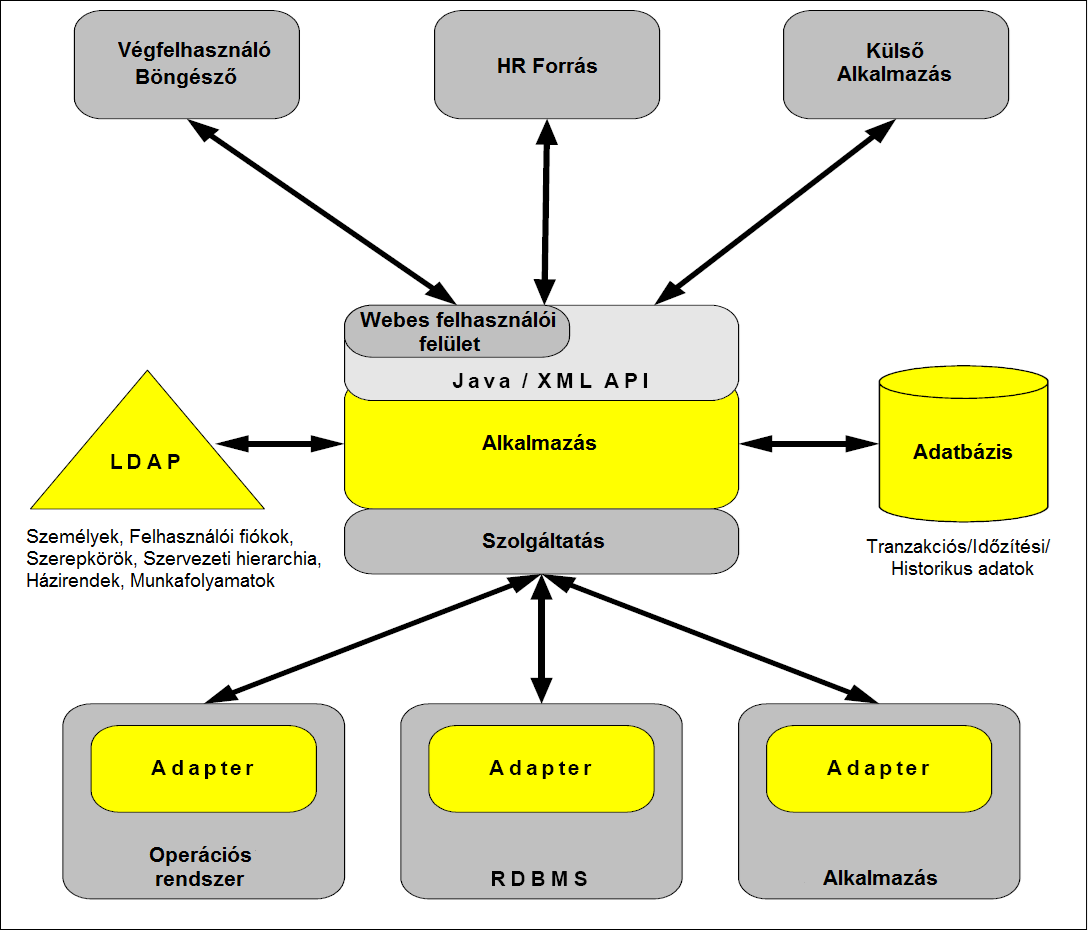
\includegraphics[width=0.5\linewidth]{figures/ISIM_promo.png}
	\caption{Az ISIM architektúrája és interfészei.}
	\label{fig:isim-promo}
\end{figure}


\subsection{Tivoli Directory Integrator - TDI}
\label{subsec:TDI}
A Tivoli Directory Integrator egy általános célú integrációs eszköz, ami lehetővé teszi több, különböző adatforrás koordinálását és integrációját.\cite{tdidoc} Mivel a legtöbb forrás más formátumot használ, és máshogy tárolja az adatot, egy ilyen integrációs lépés során szükséges bizonyos átalakításokat elvégezni az adatokon, valamint lehetséges hogy egyéb, plusz lépéseket is szükséges bevezetni, akár más adatforrások bevonásával. Ennek a procedúrának ad keretet a TDI egy grafikus fejlesztő felülettel, valamint a megfelelő Java alapú interfészekkel és kötésekkel, amelyek könnyűvé teszik új komponensek fejlesztését.

A TDI alapvető struktúrája úgynevezett assembly line-okból áll. Egy assembly line jelképez egy adat transzfert, a kezdeti adatok felolvasásától az átalakításokon át, a végső kimenet feltöltéséig. A ki- és bemeneti interakció ún. connectorokon keresztül történik, amelyek egy egységes interfészt implementálnak, és valamilyen külső adatforráshoz való kapcsolódást valósítanak meg. Minden connector, attól függően, hogy milyen műveletet végez 8 mód egyikében működik\footnote{A módok pontos leírása megtalálható a \ref{subsec:connimpl} szekcióban.}, valamint vagy aktív, vagy passzív módon dolgozik. Az előbbinél része az assembly line soros végrehajtásának, másikban nem, de külső vezérléssel működtethető.

A különböző adatforrások más-más formátumban kezelik az adatokat, így TDI minden be- valamint kimeneti műveletnél biztosít egy hozzárendelési lépést, amellyel megadhatjuk, hogy a külső attribútumok milyen belső attribútumokra legyenek leképezve. Ilyen ún. mapping lépést az assembly line-on bármikor végrehajthatunk, és emellett még számos átalakítási lépés áll rendelkezésre, mint például ciklusok vagy elágazások használata. Az assembly line-on haladó adatokat entry-k formájában kezeli a TDI.\cite{tdientry} Egy entry egy elemi objektum, ami nevesített attribútumok halmazát képes tárolni. Ilyen entry-t bármelyik scriptben létre lehet hozni, de egy általános TDI assembly line esetén 4 darab nevesített entry-t használunk:

\begin{itemize}
	\item work: Az assembly line állandó entry-je. Ezen az objektumon keresztül utazik az adat az egyes komponensek között, valamint ezen hajtják végre az adatmódosító műveletket a connector-ok.
	\item conn: Ezt az entry objektumot használják a connecot-ok a köztes adatok tárolására a célrendszerrel való kapcsolat során. Ebből az entry-ből kerülnek át az egyes mapping-ek során az adatok a work entry-be.
	\item current: Bizonyos connector-ok update módjainál elérhető változó, ami a csatlakoztatott rendszeren található adatokat tartalmazza.
	\item error: A hibakezelést végző komponensekben elérhető entry. A hibákkal kapcsolatos információkat tartalmazza.
\end{itemize}

A TDI talán egyik legfontosabb képessége a Javascriptből való testreszabhatóság. Ez azt jelenti, hogy az assembly line-on az adatokat szabadon manipulálhatjuk Javascriptes kódból, létrehozhatunk szkripteket amik a futtatás bizonyos pontjain aktiválódnak, valamint számtalan egyéb funkciót érhetünk el ezekből a programokból, mint például a logolás, paraméterek módosítása, vagy arbitrális kód futtatása.

A dolgozat szempontjából az egyik legfontosabb része a TDI-nak a connectorok, mivel a feladat része volt egy ilyen fejelsztése, ami támogatja a kommunikációt egy QRadar szerverrel, azon belül is a QRadarban található reference data objektumokkal.

\chapter{Feladat megvalósítása}
\label{ch:imp}
Mint már fentebb említésre került, a dolgozat témája részben egy valós, határidős projekt volt, így ennek megfelelően egy csapat dolgozott rajta. Ezen belül én is részfeladatokat kaptam és implementáltam, valamint részt vettem a tervezési procedúrában. 

\section{Wrapper fejlesztése QRadar-hoz}
A projekt első kihívása egy Java alapú wrapper fejlesztése volt a QRadar reference data manipulációt kezelő webes REST apijához. Későbbiekben ezen a wrapperen keresztül bonyolítunk majd minden forgalmat az átláthatóbb kód készítése céljából, ezért fontos hogy a wrapper megvalósítson minden olyan funkciót amire szükség lehet.

A fejlesztés első lépéseként tanulmányoztam a REST Api-hoz tartozó referencia dokumentációt, ami leírja mely endpointokon milyen HTTP kérések hajthatók végre, milyen paraméterekkel, milyen választ adhat és milyen státusz üzeneteket kaphatunk. Ebből az anyagból kiderült, hogy a négy reference data típushoz 4 endpoint halmaz tartozik, amelyek hasonló felépítéssel és paraméterezéssel bírnak. Egy ilyen endpoint halmazra mutat példát az alábbi felsorolás.

\begin{itemize}
	\item /sets - GET, és POST műveletet támogat. A POST-tal új reference set hozható létre, a GET metódussal pedig lekérhető a rendelkezésre álló setek listája.
		\subitem /\{name\} - GET, POST, DELETE. Az URL-ben megadott paramétert a QRadar a reference set neveként értelmezi, és ezen keresztül érhető el a set lekérése (GET), teljes törlése (DELETE), valamint egy elemi adat feltöltése (POST).
			\subsubitem /\{value\} - DELETE. Ennek az endpointnak a segítségével tudunk egy bizonyos értéket törölni a reference set-ből.
		\subitem /bulk\_load/\{name\} - POST. Az egyik legfontosabb endpoint, mivel ezen keresztül tudunk feltölteni egy olyan JSON formátumú szöveget, amellyel egyszerre több értéket is tudunk állítani egy reference set-ben (vagy más endpointok esetén más reference data-kban).
\end{itemize}

A fent felsorolt endpointok közül mindegyiket implementáltam a wrapperben, Java konvención alapuló neveket adva  a függvényeknek. Egy függvény egy működést valósít meg, és ez a működés a reference data típusának szempontjából transzparens, tehát nem szükséges külön metódust hívni egy reference set és egy reference map feltöltéséhez, hanem elég egy metódust, más paraméterekkel.

A reference data-kkal való könnyebb interakció miatt definiáltunk egy saját adatszerkezetet egy Java osztály formájában, a data típusokkal megegyező néven. Mindegyik osztály egy ReferenceData navű absztrakt ősosztályból származik, ami egy egységes interface-t biztosít a leíró adatok, mint például a típus, az adatok típusa, lekéréséhez. Ennek a ReferenceData-nak a leszármazottai a konkrét reference típusokat megvalósító osztályok. Mindegyik osztály rendelkezik egy, a saját maga által reprezentált struktúrának megfelelő tárolóval, amely tárolja az adott reference data adatait. Mivel az integráció során többnyire szöveges, vagy azzá könnyen átalakítható adatokkal dolgozunk, és a QRadar irányába is JSON formátumban továbbítjuk az adatokat, így kézenfekvő mindet szövegként tárolni. A tárolókhoz használt kollekciók pontos típusa, valamint az implementációhoz használt architektúra leolvasható a mellékelt ábráról \ref{fig:referencedata}. 

Lehetséges lenne más formátumban tárolni az adatokat, mint például egy Java alapú JSON reprezentációban, JSONObject-ben, vagy akár egy hosszú karakterláncként is, ám ezzel elvesztenénk a Java beépített kollekciói által nyújtott funkciókat, mint például az iterációt, vagy a tartalmazás ellenőrzését. Ezek mind nélkülözhetetlen funkciók a könnyű fejlesztés érdekében, valamint a megfelelő teljesítmény biztosítása szempontjából is fontosak, amire később látunk majd példát. 

\begin{figure}
	\centering
	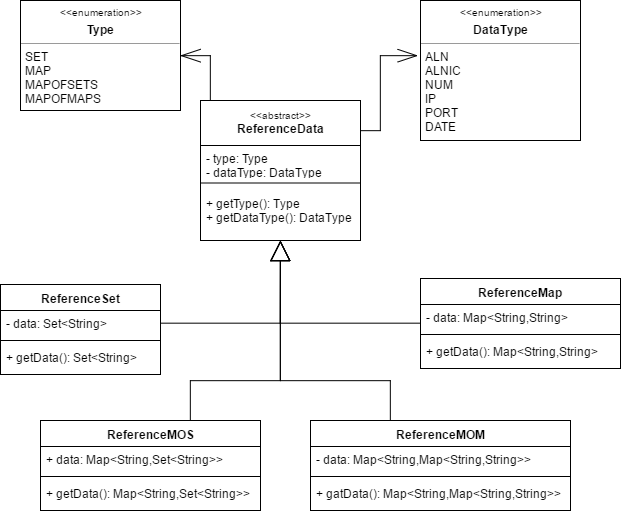
\includegraphics[width=0.7\linewidth]{figures/ReferenceData}
	\caption{A ReferenceData osztály és leszármazottainak felépítése}
	\label{fig:referencedata}
\end{figure}

A wrapper fejlesztése közben külön kihívást jelentett a QRadar REST api-val való kommunikáció megvalósítása. A QRadar ugyanis csak HTTPS forgalmat fogad el, TLS segítségével, ezért egy, a QRadar által generált tanusítványt kellett hozzáadni minden olyan környezethez, amely a wrappert használta. Ez a két külön architektúra esetén a WebSphere és a TDI tanusítvány könyvtárát jelentette, és ez egy olyan követelmény, ami a wrapper későbbi használata esetén is szükséges. Emellett a QRadar megköveteli, hogy a REST API-jához csatlakozó kliensek használjanak egy, a QRadar által előre generált token-t, amit minden híváskor fel kell küldeniük. A wrapper osztály ezt konstruktorában kéri, és automatikusan minden kérésnél elküldi. A TLS kapcsolat biztosítja a szerver hitelességét, míg a token a szerver számára hitelsíti az API-t használó klienst, így összeségében a kommunikáció kölcsönösen hitelesített.

Magának a HTTP forgalomnak és a REST hívásoknak a lebonyolítására az Apache Wink\footnote{\hyperlink{Apache Wink}{\url{https://wink.apache.org}}} framework-öt használtam. Ez egy egyszerű Java alapú framework, melynek része egy JAX-RS kompatiblis szerver, és egy kifejezetten REST hívások lebonyolítására kiélezett HTTP kliens. A projektben a kliens komponens RestClient osztályát használtam, valamint a frameworkkel együtt érkező JSON4J csomagot, a JSON inputok parse-olására és a szöveges outputok generálására. A fejlesztés közben külön kihívást jelentett a JSON4J csomag megfelelő osztályainak használata, valamint egymásba ágyazása. Ez a csomag ugyanis két osztályt bocsájt rendelkezésre a JSONObject valamint a JSONArray formájában. Az object osztály reprezentálja a map típusú, míg az array a tömb típusú struktúrákat. Ez annyiban nehezítette a fejlesztést, hogy a különböző ReferenceData leszármazottak közt nem lehetett egységes parseolást használni, hanem a többszörösen egymásba ágyazott kollekciók esetén több lépcsős iterációt kellett használni a JSON felépítéséhez. Ez túl nagy adathalmazoknál lassabb működést eredményezhet.

A wrapper a különböző reference data-k transzparens kezelésén túl egyéb funkciókat is ellát, mint például segéd funkciók biztosítása, vagy a hibák egységes kezelése. Ilyen segéd funkciók a különböző adattranszformációk a használt típusok és a JSON formátum között, vagy például különböző ellenőrzések egy reference data létezésére, vagy egy aszinkron törlés lefutására. A hibakezelés menedzselésére a wrapper egy saját kivétel osztályt definiál, ami minden, a sikeres lefutástól eltérő esetben (akár belső hiba, akár a QRadarral való kommunikáció közben fellépő hiba) eldobásra kerül. Ez az objektum tartalmaz egy szöveges üzenetet, ami a hiba okára utal, valamint egy státusz kódot, ami ha HTTP kommunikáció közbeni hiba történt, annak a kódját tartalmazza, ha belső működésbeli hiba (például parse-olási hiba) akkor egy 0-nál kisebb számot tartalmaz. Ez egységesen és könnyen használhatóvá teszi a felsőbb rétegek számára, ahol például logolást kezeljük, mert egyértelmű, hogy a hiba milyen forrásból adódott. A saját kivétel típus pedig tovább könnyíti a hibák elválasztását, főleg ha a wrapper-t egy nagyobb framework-ben használjuk.

\section{TDI Integráció megvalósítása}
% Mod
A TDI alapú megoldás célja egy olyan keret, és hozzá tartozó use case-ek kidolgozása, amely lehetőséget ad az ISIM és QRadar közti integrációs feladatok gyors, hatékony és egyszerű megvalósítására. 
A TDI már létező LDAP és adatbázis (JDBC) connectorral rendelkezik, ezért az ISIM adatforrásként való használata gyári komponensekkel oldható meg. A QRadar API használatához viszont új connector fejlesztésére volt szükség.
Mivel a TDI által nyújtott keretrendszerbe illeszkedik a megoldás, így képes használni az általa nyújtott számos lehetőséget, például a már létező connector-okat sokféle rendszerhez, valamint a use case implementációk alapján később könnyedén készíthetők új megoldások olyanok által, akik járatosak a TDI használatában. 

A megvalósításhoz szükség volt elsősorban egy connector létrehozására, majd ezt felhasználva implementáltam több lekérdezés típust, általunk, valamint az ügyfél által definiált esetekre.
% Mod
 
\subsection{QRadar connector fejlesztése TDI-hoz}

A TDI alapú megoldás első lépése egy connector fejlesztése volt a TDI és a QRadar közti integrációhoz. Ehhez segítségemre volt a hivatalos útmutató connector fejlesztéshez, ami az IBM oldalán megtalálható. Egy saját connector fejlesztése TDI alatt abból áll, hogy létrehozunk egy új Java osztályt ami implementálja a megfelelő, TDI által specifikált interfészt, ennek metódusain belül elkészítjük a kívánt üzleti logikát, majd egy xml leíró fájllal együtt, a megfelelő struktúrában becsomagoljuk azt egy JAR fájlba, amit a TDI által használt könyvtárak egyikébe másolunk. 

Egy connector-nak hat működési módja lehet, amit a feljebb említett dokumentum specifikál. Ezek a következők:


\begin{itemize}
	\item Iterator - Végigiterál az adatforrás elemein, azokat felolvassa, és az assembly line rendelkezésére bocsájtja.
	\item AddOnly - Az assembly line-on érkező adatokat hozzáadja az adatforráshoz.
	\item Lookup - Egy kritérium alapján keresést hajt végre az adatforráson és kiválasztja a kritériumra illeszkedő elemet vagy elemeket. Jellemzően több adatforrás elemeinek illesztésére használatos.
	\item Delete - Az assembly line-ról kapott összes elem esetén a megadott kritériumot felhasználva megkeresi az elemet, és ha megtalálta, törli azt. Lehetőség van olyan felparaméterezésre is, amely egyszerre több elemet töröl.
	\item Update - Már meglévő adatok módosítását végzi. Előbb  megkeresi a megadott kriétérium alapján a rekordokat, ha talált ilyen elemet, akkor összehasonlítja az assembly line-on érkező elemmel, és elvégzi a szükséges módosításokat. Ha nem talált megfelelő elemet, akkor hozzáadja újként.
	\item Delta - Egy különleges mód, melyhez szükség van további, ilyen módot támogató elemekre az assembly line-on. A felolvasott adatokat összehasonlítja egy külső tárolóban (ún. delta store) tárolt elemekkel, és a két elem differenciáiból delta műveleteket képez, amiket végrehajt a célrendszeren. Eltárolja a kezelt elemek legutóbb használt verzióját, és csak az újonnan beolvasott elemekhez képesti különbséget hajtja végre.
\end{itemize}

Egy connector nem feltétlenül támogat minden módot, a támogatni kívánt módok határozzák meg, hogy a fejlesztendő connector-nak milyen metódusokat kell implementálnia a megfelelő működéshez. 
Például az AddOnly mód csak az Initialize, putEntry, és a terminate metódusokat használja, így ha a connector csak ezt akarja használni, elég ezeket implementálni. Ezzel szemben például az Update mód ezeken felül használja a findEntry, és a modEntry metódust is. Minden connector a saját logikáját definiálja, amivel megvalósítja az adott célrendszeren az absztrakt módon megfogalmazott műveletet. Egy JDBC connector például adatbázis parancsokkal valósítja meg a fent definiált műveleteket egy kapcsolaton keresztül. Jelen esetben egy REST API-n keresztül elérhető a kommunikáció a célrendszerrel, így a connector szabványos HTTP kéréseket használ. A fejlesztés során megvalósításra került az összes fent említett mód.

% Mod
Első lépésként tehát elkészítettem egy QRadarReferenceDataConnector osztályt, ami örököl egy generikus ősosztályból, ami már előre megvalósít olyan metódusokat a TDI által használt ConnectorInterface-en, amelyek nem kifejezetten connector specifikusak, hanem generikus feladatokat látnak el, például konfigurációs fájlok beolvasása vagy paraméterek beállítása.
% Mod

Az implementációs döntések megértéséhez fontos ismerni egy connector életciklusát. A connector létrejöttekor meghívódik a konstruktora, de ez a dokumentációban leírtaknak megfelelően nem szabad hogy paraméter és egyéb beállításokat tartalmazzon, mert a példány már létrejöhet az előtt, hogy a szükséges paraméterek beolvasásra kerültek. Ez azért történhet meg, mert ezt a konstruktort használja a TDI grafikus felülete a kezdeti beállítási és paraméterezési felület elkészítéséhez. A konfiguráló, valamint az erőforrás foglaló műveletek ezért az Initialize metódusban kaptak helyet, ami az assembly line futás elején hívódik meg. A connector objektum egészen az assembly line végéig életben marad, majd annak végén mielőtt a destruktor meghívódna, lefut az objektum terminate metódusa. Erre azért van szükség, hogy a connector megfelelően felszabadíthassa az általa foglalt erőforrásokat.

A connector életciklus ismeretében, valamint a QRadar és a REST API-jának működése és telejsítménye miatt az alábbi megoldás mellett döntöttünk: az assembly line futása közben nem azonnal kerülnek fel az adatok a QRadar megfelelő reference data-jába, hanem azok először a connector egy változójában akkumulálódnak, és az életciklus végén, a terminate metódus segítségével kommitálódnak. Két ilyen változót használtam, egyet a törlendő, egyet az újonnan hozzáadandó elemek tárolására. A megvalósítás valamint a wrapper használata miatt adott volt, hogy ezeknek az akkumulátor változóknak a megvalósítását a QRadarApiWrapper mellé fejlesztett ReferenceData osztály, valamint leszármazottjai szolgáltassák.

A connector használatához szükséges annak megfelelő felparaméterezése. Erre a TDI a grafikus fejlesztői felületén ad lehetőséget, ahol a connector által definiált paraméterek megadására beviteli mezők állnak rendelkezésre. Minden connectornak más paraméterekre van szüksége, ezt egy tdi.xml fájl megadásával írhatjuk le, amit a connector osztályt tartalmazó JAR fájlba csomagolunk be. Ezeket aztán a GUI segítségével megadhatjuk kézzel, paraméter fájl használatával, Javascript kóddal vagy helyettesítéssel, ami akár az aktuális entitás értékeit is felhasználhatja. A QRadar connector működéséhez legalább a QRadar példány elérhetőségét, a hozzá tartozó token-t, a reference data nevét, típusát, valamint az általa használt adat típusát meg kell adni.
% Mod
Végeredményképp létrehoztam a felvázolt működésnek megfelelő connector-t, ami képes a paraméterezés alapján megadott QRadar példánnyal felvenni a kapcsolatot, számára adatot feltölteni, módosítani, törölni. Ez bármilyen assembly line-ban használható, későbbi projektek során is.

\subsection{Connector tesztelése}
%concept, legyen ilyen fejezet? kell ide?
A fejlesztés következő lépése az elkészített connector tesztelése volt, valamint a helyes működés ellenőrzése. Az ennek során szerzett tapasztalatokra építve készítettem el a \ref{sec:queryk}. \nameref{sec:queryk} fejezetben leírt integrációs feladatokat.

A teszteléshez kézzel megadtam néhány inputot, melyeket megkíséreltem feltölteni a connector segítségével egy Reference Data-ba, majd ezeket ellenőriztem a QRadar belső menüjének használatával.
 A  \ref{fig:conntest1}-es Ábrán látható, hogy egy Javascript blokk formájában feltöltöm az assembly line fő változójának értékét egyedileg definiált szövegekkel. A bal oldalon látható a teszt Assembly line, ami a feltöltő script-ből áll, a QRadar Connectorból, valamint egy ciklus vezérlőből, ami az összes string értéket egyesével továbbítja a QRadar Connector felé. A  \ref{fig:conntest2} Ábrán látható a QRadar Connector felkonfigurálása.
 
 Az assembly line futtatása után, a folyamat eredményességét a QRadar Reference Set módosító felületén keresztül ellenőriztem. Az eredmény a \ref{fig:qradartest1} Ábrán látható. %Látszik, hogy az összes kézzel definiált szöveg felkerült az adott set-be. A

\begin{figure}[b]
	\centering
	\begin{minipage}{0.45\textwidth}
		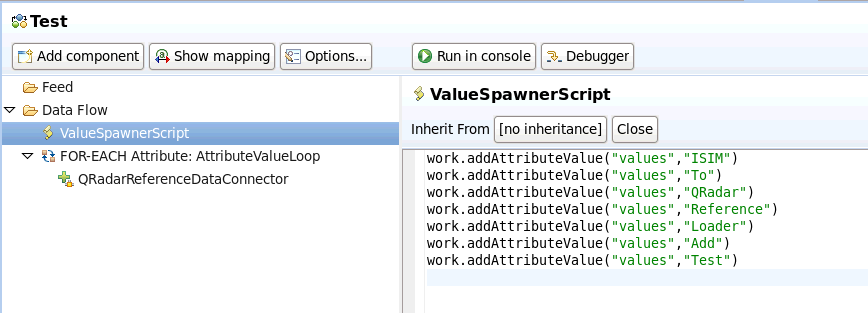
\includegraphics[width=0.9\linewidth]{figures/conn_test/connTest1}
		\caption{Adatok kézi megadása}
		\label{fig:conntest1}
	\end{minipage}
	\begin{minipage}{0.45\textwidth}
		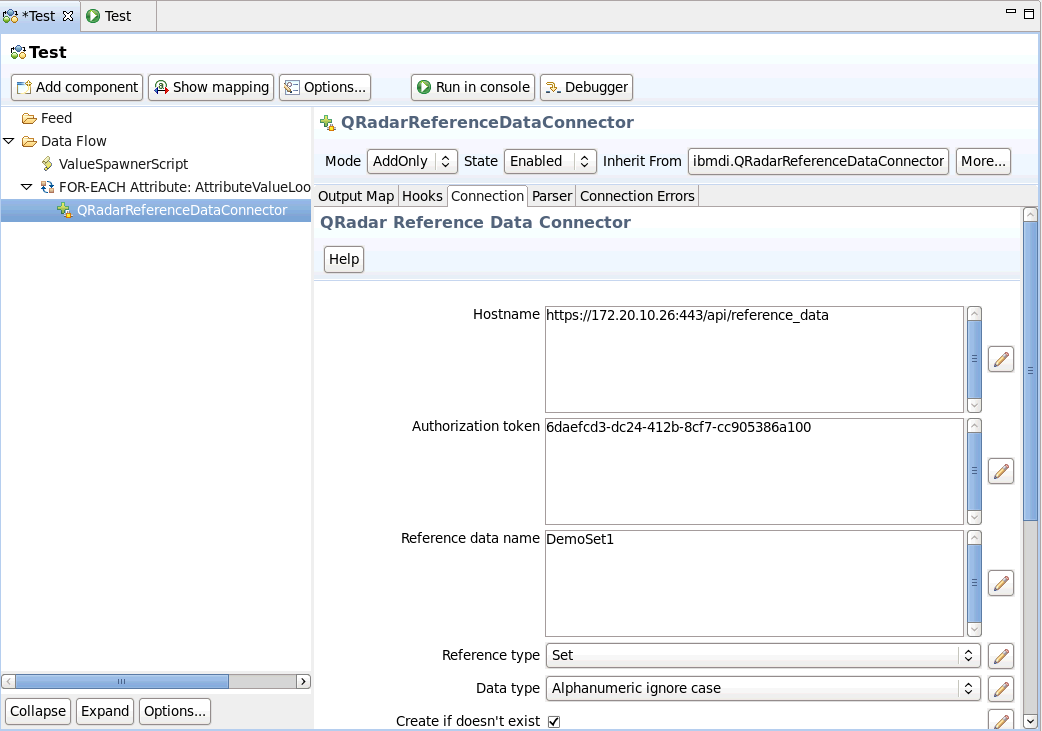
\includegraphics[width=0.9\linewidth]{figures/conn_test/connTest2}
		\caption{Connector konfigurációja}
		\label{fig:conntest2}
	\end{minipage}

\end{figure}
\begin{figure}
	\centering
	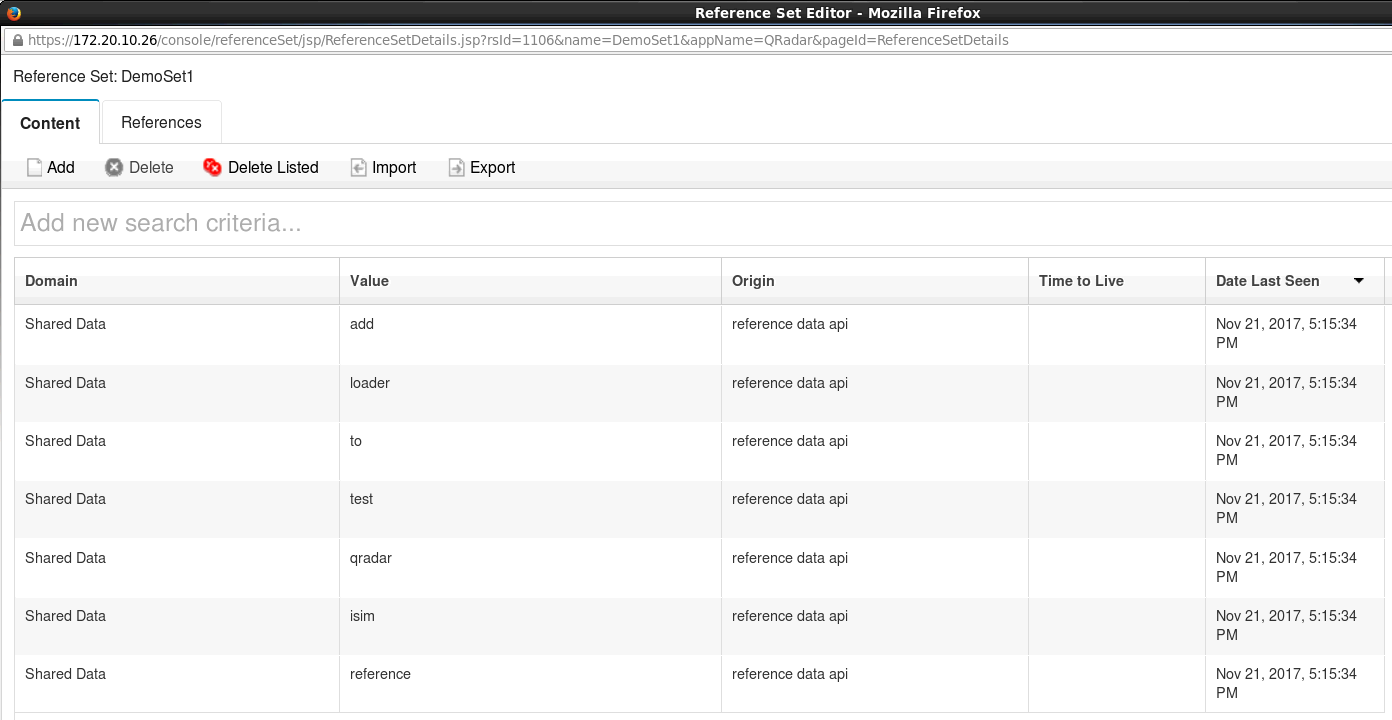
\includegraphics[width=0.9\linewidth]{figures/conn_test/qradarTest1}
	\caption{Feltöltött adatok}
	\label{fig:qradartest1}
\end{figure}
A hozzáadáson kívül ellenőriztem a connector további műveleteit is: a törlést, a módosítást, az iterációt és a deltát.
\todo függelék képernyőképek a többi módról?



\section{WAS integráció megvalósítása}

Ennél a megoldásnál a cél egy robusztus alkalmazás megalkotása volt, ami jól illeszkedik egy nagyvállalati környezetbe, valamint működés és üzemeltetés szempontjából is összhangban van a hozzá kapcsolódó IBM-es termékekkel. Az előző szekcióban ismeretett TDI alapú megoldás ugyan ellátja a szükséges feladatokat, a fejlesztés egyszerű és gyors, de a használt technológiából adódik, hogy más területeken hátrányban van egy különálló, vagy akár egy menedszelt környezetben futtatott alkalmazással szemben. Ezeket a hátrányos tulajdonságokat hivatott áthidalni a Websphere alapú megoldás.

A WebSphere alapú alkalmazás fejlesztésének főbb motivációi:
\begin{itemize}	
	\item A magas rendelkezésre állás, elosztott futtatás, egységes alkalmazásmenedzsment biztosítása.	
	\item Jogosultságkezelés és auditálhatóság megvalósítása. 
	\item Fejlesztői és üzemeltetői feladatok szétválasztása, valamint az üzemeltetési feladatok felhasználói felülettel való támogatása.
\end{itemize}

A felsorolt funkciók TDI-vel történő megvalósítása valamilyen külső megoldást kívánna, ami növelné az alkalmazás beállítási és karbantartási komplexitását, mivel ezekre is figyelmet kell fordítanunk, ezeket is ellenőriznünk kellene esetleges hibák felmerülésekor. További probléma, hogy a TDI alapú megoldás testre szabhatósága bizonyos kereteken túl nem, vagy nagyon nehezen megvalósítható. Ilyen például a felhasználói felület kérdése. A TDI alapú megoldásnál adottak az opciók: a Configuration Editor, azaz a fejlesztői alkalmazás használata, vagy a megfelelő parancssoros lehetőségek használata. Ha saját felületet akarunk készíteni, akkor nem csak annak a fejlesztését kell megvalósítanunk, de a TDI által biztosított interfészekkel való kommunikációt is. Ezzel szemben egy saját alkalmazás, menedzselt környezetben futtatva, az adott alkalmazásszerver által nyújtott lehetőségekkel együtt, a legtöbb felsorolt problémára megoldást nyújthat. 

%Az automatizált futtatást biztosítja a szerver által nyújtott ütemező, a naprakészséget és a magas rendelkezésre állóságot a szerver architektúrája és infrastruktúrája. Emellett megvalósíthatunk egyedi megoldásokat is, mint például egy egyedi logikát, ami biztosítja az elakadó szinkronizációs feladatok és az inkonzisztenciák korrigálását. A technikai és hozzáférési információkat, valamint az elosztott futtatást szintén nem kell alkalmazás szinten kezelnünk, mert a szerver tárolhatja a cache-elhető információkat és erőforrásokat, akár egy poolozott megoldással, amiket szükség esetén az alkalmazás rendelkezésére bocsájt, akár elosztottan, több példány számára is. 

A Websphere alapú alkalmazás a fenti területkre az alábbi módon kínál megoldást:
\begin{itemize}
	\item Futtatásra használhatjuk a WebSphere által kínált beépített ütemezőt, ami az általunk megadott szabályok szerint végrehajtja a feladatokat.
	
	\item Az paraméterek, valamint a feladatok elosztott végrehajtását képes a szerver kezelni, így a magas rendelkezésre állóságot elég ha a szerver szintjén biztosítjuk. Az adatok naprakészen tartásához emellett készíthetünk egyedi logikát, ami szükség esetén változtat a futtatandó feladatok során.
	
	\item Mivel az alkalmazás nem közvetlenül, hanem a szerver által biztosított kapcsolatokon keresztül csatlakozik a célrendszerhez, a költséges erőforrások poolozása könnyen támogatható, valamint biztonsági szempontból is elég a szervert biztosítani.
	
	\item Egy saját fejlesztésű, egyedi felülettel könnyen szétválaszthatók a fejlesztői, és a felhasználói feladatok a rendszer használatánál. A fejlesztő megvalósított néhány általános use case-t, amelyet a felhasználó később elér, hogy saját igényei szerint felparaméterezze, és használja őket. 
	
\end{itemize}

\todo UML diagramok?
\subsection{Architektúra tervezése}

Mivel az alkalmazás egy projekt részeként valósult meg, többen dolgoztunk rajta, ez különösen fontossá tette az architektúra átgondolását és alapos megtervezését. 

A cél egy olyan alkalmazás fejlesztése volt, ami mind a jövőbeni fejlesztők, mind az üzemeltetéssel foglalkozó személyzet számára könnyen használható. Jelen esetben a fejlesztők alatt elsősorban azokat a személyeket értem, akik majd későbbiekben új lekérdezés (query) típusokat készítenek a rendszerhez. Ezek a személyek mélyebb ismeretekkel rendelkeznek a rendszerrel kapcsolatban, ám fontos, hogy számukra is egy könnyen használható interfészt biztosítsunk. Emellett fontos, hogy az új lekérdezés típusok könnyen, az alkalmazás minimális -- vagy optimális esetben semmilyen -- módosításával bevezethetők legyenek. Ezzel jól szétválasztható a fejlesztők és az üzemeltetők számára szükséges tudás, mivel egy már kész, új típust egy, a rendszer belső működéséhez kevésbé értő ember is gyorsan be tud vezetni. Üzemeltetői részről egy könnyen használható felület biztosítása volt a cél, ami egyértelmű tudósítást ad a rendszer állapotáról, és megkönnyíti új lekérdezések konfigurálását, azok helyes felparaméterezését.

A tervezésnél az alábbi döntéseket hoztuk:

\begin{itemize}
	\item Egységes, moduláris lekérdezésrendszer
	\begin{itemize}
		\item A különböző lekérdezés típusok egy közös interfészt implementálnak.
		\item Minden ténylegesen lefutó lekérdezés egy lekérdezés típusból, és annak a felparaméterezéséből áll. Ezeket egy táblában szerializálva tároljuk, ahonnan az ütemező felolvassa, és futtatja őket.
	\end{itemize}
	
	\item Két ütemező, külön időzítéssel, egy az ISIM lekérésekhez, egy a QRadar szinkronizációhoz.
	
	\item Kétfázisú lekérdezések, több lehetséges állapottal (Lsd.: \ref{fig:refloaderstates} Ábra)
	\begin{itemize}
		\item Minden lekérdezés két fázisból áll: egy ISIM irányú lekérési fázisból, és egy feltöltési fázisból a QRadar felé
		\item A lekérdezés létrejöttekor egy kezdeti állapotban van.
		\item Az ütemező elindítja a lekérdezést, ekkor IDM\_SYNC\_RUNNING állapotba kerül, és elkezd futni a definiált ISIM lekérdezés.
		\item Ha a folyamat sikeres volt, IDM\_SYNC\_COMPLETED állapotba kerül, ha nem, akkor IDM\_FAILED-be
		\item Az IDM\_SYNC\_COMPLETED állapot után a lekérdezés vár, amíg az ütemező el nem indítja a QRadar irányú szinkronizációt, vagy újra sorra nem kerül az ISIM ütemező számára.
		\item A QRadar szinkronizáció futása ha sikeres, akkor COMPLETED állapotba kerül a lekérdezés. Ezt az állapotot nevezzük a sikeres végállapotnak.
		\item Ha a QRadar szinkronizáció nem volt sikeres, akkor QRADAR\_SYNC\_FAILED állapotba kerül. Ekkor a lekérdezés vár, hogy a két ütemező közül valamelyik elindítsa az egyik feladatát.
	\end{itemize}

	\item Lekérdezések eredményeinek tárolása, delta számolás
	\begin{itemize}
		\item Egy lekérdezés futtatása közben, minden sikeresen lefuttatott fázis után szerializáljuk az eredményt egy SQL adatbázisba. Emiatt ha az alkalmazás hibára futna, vagy újraindulna két fázis között, a lekérdezés eredménye megmarad.
		\item A QRadar-ra legutóbb feltöltött állapotról tárolunk egy lokális verziót, amit összehasonlítunk az ISIM lekérdezés eredményével. Ha változás történt, akkor csak a két állapot különbségét töltjük fel.
		\item Ha a különbség feltöltése közben hibára futunk, feltételezhetjük hogy a rendszeren kívülről valaki módosítást hajtott végre, és a lokális változat már nincs szinkronban. Ekkor egy teljes feltöltést végzünk az adatokkal.
	\end{itemize}

	\item Egyedi felhasználói felület fejlesztése
	\begin{itemize}
		\item Olyan felület, amelyen egyszerűen láthatók a rendszerben megtalálható, már felkonfigurált lekérdezések, valamit könnyen és gyorsan új lekérdezéseket konfigurálhatunk fel.
		\item Lekérdezések létrehozásának könnyítése sémafelderítéssel, aminek a segítségével a rendszerben található service-ek, organizációs egységek, szerepkörök, stb... listákból kiválaszthatók.
	\end{itemize}
\end{itemize}

\begin{figure}
	\centering
	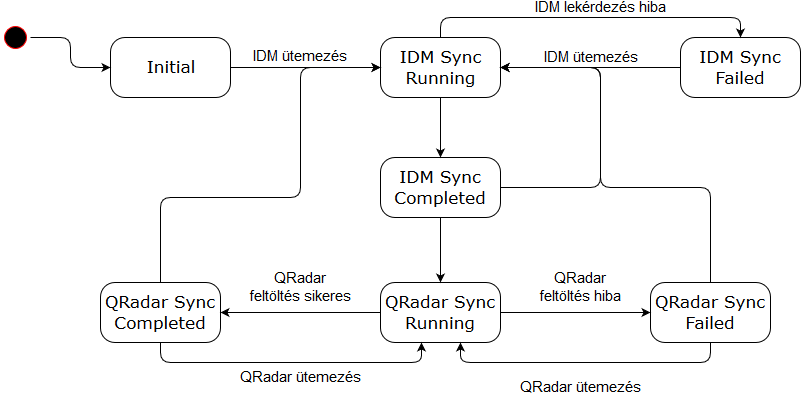
\includegraphics[width=0.9\linewidth]{figures/refloader_states}
	\caption{Egy lekérdezés futásának állapotai}
	\label{fig:refloaderstates}
\end{figure}


\section{Query-k implementációja} \label{sec:queryk}
% Mod
A koncepció, valamint a fejlesztett megoldások tesztelésére az alábbi use-case-eket definiáltuk:

\begin{itemize}
	\item Felhasználói fiókok egy adott menedzselt rendszeren
	\begin{itemize}
		\small
		\item Felhasználása: Ellenőrizhető, hogy az eseményben jelzett fiók az ISIM által kezelt e, és ha nem, az okot adhat biztonsági riasztásra.
		\item Megvalósítás: Szűrés az LDAP-ban található felhasználói fiókokra, aszerint, hogy melyik service-hez tartoznak.
	\end{itemize} 
	\item Inaktív felhasználókhoz tartozó fiókok
	\begin{itemize}
		\small
		\item Felhasználása: A SIEM riasztást adhat ha olyan tevékenység történik, ami ezekhez a felhasználói fiókokhoz kapcsolódik. Ezek elsősorban akkor következhetnek be, vagy akkor jelenthetnek kockázatot, ha a felfüggesztés a felhasználó fiókjaira valamiért nem érvényesült, és képes használni. De felhasználható visszamenőleg is, irreguláris tevékenységek keresésére.
		\item Megvalósítás: LDAP szűrés az összes inaktív felhasználóra, majd szűrés az összes fiókra, az alapján, hogy tulajdonosa e az egyik megtalált felhasználó e.
	\end{itemize}
	\item Felfüggesztési eljárás alatt álló felhasználók fiókjai
	\begin{itemize}
		\small
		\item Felhasználása: A SIEM riasztást adhat ezen felhasználói fiókok detektálásakor. Biztonsági szempontból első sorban azért érdekes, mert a felfüggesztett személyeket általában okkal, és jogvesztéssel együtt függesztik fel (bírósági vizsgálat, kirúgás, stb), emiatt lehetséges hogy a felfüggesztés célpontja bosszúból valami ártalmas tevékenységet követ el.
		\item Megvalósítás: Adatbázis keresés a jelen pillanatban futó felfüggesztési folyamatokra, majd az ebből kinyert felhasználó azonosítója alapján LDAP szűrés az összes fiók között.
	\end{itemize}
	\item Törlési folyamat alatt álló felhasználói fiókok
	\begin{itemize}
		\small
		\item Felhasználása: Az előző esethez hasonlóan a törlés is egy jogfosztó művelet, ami ha nem atomi módon fut le, hanem például valamilyen kommunikációs hiba miatt megakad, akkor egy ablak nyílik a rosszindulatú felhasználók számára, hogy kárt tegyenek a rendszerben.
		\item Megvalósítás:  Adatbázis keresés a jelen pillanatban futó felhasználói fiók törlési folyamatokra.
	\end{itemize}
	\item Árva fiókok
	\begin{itemize}
		\small
		\item Felhasználása: Ezek olyan fiókok, melyek nem köthetők valós, a rendszerben kezelt személyhez. Ilyenek lehetnek például a rendszer által menedszelt technikai fiókok, vagy olyanok, amik korábban valós felhasználókhoz tartoztak, de valamiért megmaradtak a szétválás után is. Ezek komoly biztonsági rést jelenthetnek, elsősorban ha például hozzáférnek kritikus rendszerekhez, de megmaradt a alapértelmezett jelszavuk, vagy nem alkalmazták rájuk a jelszó házirendeket.
		\item Megvalósítás: Mivel az ISIM az LDAP adatbázisában ezeket a fiókokat külön tárolja, elég ezt lekérnünk. Majd a kinyert adatok alapján hozzárendeljük őket a megfelelő service-hez, és annak a megfelelő azonosítójához.
	\end{itemize}
	\item Egy menedzselt rendszeren a megadott csoportokba tartozó felhasználói fiókok
	\begin{itemize}
		\small
		\item Felhasználása: A legtöbb informatikai rendszeren létezik valamilyen felhasználói fiók csoportosítás, ami többnyire az azonos jogkörrel rendelkező fiókokat definiálja. Ha megvannak egy adott csoportba tartozó fiókok nevei, akkor könnyen létrehozhatunk irregularitás detektáló szabályokat, mint például ha a privilegizált felhasználók munkaidőn kívül lépnek be, ami jelentheti akár a fiókjuk kompromittálódását is.
		\item Megvalósítás: LDAP szűrés az előre definiált csoport attribútum alapján, az adott service-hez tartozó felhasználói fiókokon.
	\end{itemize}
	
\end{itemize}
\section{QRadar esemény küldő fejlesztése}
A feladat motivációja, az eddig felsorolt problémákhoz hasonlóan, a QRadar monitorozási és detektálási hatékonyságának bővítése az ISIM segítségével. Az előző két implementált megoldásban az ISIM-ben tárolt felhasználói adatok egy részhalmazát tettem elérhetővé a QRadar szabályrendszere számára, mert ezek a plusz információk hasznosak lehetnek az események értelmezésében. Ezzel szemben ennél a megoldásnál az ISIM mint log forrást illesztettem a QRadarhoz. Egy ilyen megoldás már rendelkezésre állt, de az a QRadar JDBC csatlakozóját használja, ami limitált képességekkel bír (például nem join-olhatók vele táblák), és csak az ISIM-ben található audit információkat kezelte.

A fejlesztett megoldás célja más, nem audittal kapcsolatos információk küldése a QRadar számára log formájában. Ezek is fontosak lehetnek biztonsági eseményeknél, hiszen például az ISIM-ben futó/futott folyamatok információit felhasználva új incidenseket vehetünk észre. Ilyenek lehetnek jelszó változtatások (például egy széles jogkörrel rendelkező felhasználó jelszó cseréje nem várt időpontban), az ISIM szabályrendszerének változása, vagy például kézi jóváhagyás műveletek. 

A folyamatokkal kapcsolatos információkat az ISIM a saját DB2 adatbázisában tárolja. Minden folyamathoz tartozik egy rekord a PROCESS nevű táblában. Attól függően hogy az adott folyamat pontosan hogy van definiálva, lehet hogy más folyamatok is meghívódnak egy futás közben. Az egyes folyamatok konkrét implementációjával kapcsolatos információk az ACTIVITY táblában, míg a folyamat lefutásával kapcsolatos audit események a PROCESSLOG táblába kerülnek. Az események generálásakor elsősorban ezzel a három táblával dolgoztam.

A felsorolt táblákból kinyerhetők a folyamattal kapcsolatos technikai információk, mint a folyamat típusa, kezdeti ideje, általa hivatkozott egyéb folyamatok és activity-k. Emellett viszont olyan adatokat is tárolnak a táblák, amik a folyamatban résztvevő személyeket azonosítják. Ha ezeket az adatokat képes feldolgozni a QRadar oldali esemény fogadó, akkor az előzőekben ismertetett megoldás által feltöltött adatok segítségével kialakíthatók olyan szabályok, amik fontos incidenseket detektálhatnak.
 
\subsection{TDI alapú syslog küldő fejlesztése}
Az ISIM-ben található adatok feldolgozására, és ezekből syslog események generálására a már az előzőekben bemutatott TDI keretrendszert használtam. Ez kézenfekvőnek tűnt, mivel a TDI biztosít connectorokat mind az ISIM DB2 adatbázisa irányába, mind a syslog események generálásához és küldéséhez. Előbbire a Java JDBC protokollt használó JDBC connector-t, utóbbira a beépített Log connector-t, ami sok különböző standard logoló motor mellett a syslog-ot is támogatja. 

A fejlesztés első lépése a táblák és a bennük található adatok felmérése volt. Ez alapján az alábbi következtetésekre jutottam:

\begin{itemize}
	\item A PROCESS tábla az egyes folyamatok operatív információit tartalmazza. 
	\begin{itemize}
		\item A legfontosabb információk itt találhatók, többek közt: folyamat indítója; folyamat alanya; organizációs egység, amelyben fut; folyamat típusa és eredménye; indulási és befejezési időpont
	\end{itemize}
	\item Az ACTIVITY tábla sorai az egyes folyamatokhoz tartozó elemi akciók információit tartalmazza.
	\item A PROCESSLOG tábla a folyamat egyes lépéseinek a kiegészítő és audit információit tartalmazza.
	\item A három tábla közül a PROCESSLOG tábla tartalmazza az legkisebb felbontásban az folyamattal kapcsolatos információkat.
	\item A folyamatban résztvevő felhasználókkal kapcsolatos legfontosabb adatok a PROCESS táblában találhatók.
\end{itemize}

Ezek alapján megvalósítottam az adatok kigyűjtését a TDI segítségével. A lekérést egy 3 táblából álló join művelettel végeztem el, melyben a PROCESSLOG táblát a PROCESS táblával a PROCESS\_ID oszlopon keresztül, az ACTIVITY táblát pedig az ACTIVITY\_ID oszlopon keresztül kötöttem össze. A teljesség kedvéért mindegyik tábla mindegyik mezőjét kigyűjtöttem, további felhasználási célra. Mivel ez a TDI-ban ütközést okozott az azonos nevű mezőkön, ezért minden oszlopot a tábla nevével prefixáltam.

A következő lépés az adatok átalakítása volt a QRadar számára könnyen kezelhető formára. Mivel a feldolgozás egyik módja a reguláris kifejezések használata, így kézenfekvő volt egy olyan struktúra kialakítása, amire jól illeszthetők ilyen kifejezések. Emiatt végül az alábbiak mellett döntöttem:

\begin{itemize}
	\item Az összes attribútum összefűzése egy folytonos karakterlánccá.
	\item Az összes attribútum értéke elé az adott attribútum nevének hozzáfűzése. Például a PROCESSLOG tábla EVENTTYPE mezőjénél ez az alábbi formátumot eredményezte: PL\_EVENTTYPE={érték}
	\item Az egyes attribútumok elválasztása pontosvesszővel. Azért erre a karakterre esett a választásom, mert ezt gyakran használják ilyen célra, például az LDAP konvenciók szerint is, és pont emiatt az LDAP attribútumok értékében egy tiltott karakter, és bár közvetlenül relációs adatbázisból szelektálunk, ezek a táblák többnyire az LDAP adatbázisból kinyert, vagy ott is tárolt információkat tartalmaznak.
	\item Az új sor karakterek eltávolítása, valamint a pontosvesszők \todo kieszképelése az attribútumok értékeiből.
\end{itemize} 

%Ebből tehát ehhez hasonló sorok adódtak:

%RÖVIDTÁBLANÉV\_OSZLOPNÉV=ÉRTÉK;RÖVIDTÁBLANÉV\_OSZLOPNÉV=ÉRTÉK;RÖVIDTÁBLANÉV\_OSZLOPNÉV=ÉRTÉK;...


A generálás utolsó lépése a sorok felküldése volt syslog protokollon keresztül a QRadar megfelelő fogadó interfészére. Ehhez a beépített Log connector-t használtam, egy egyedileg konfigurált Log4J logger segítségével. Az egyedi konfiguráció definiálja, hogy a beépített syslog logger legyen a használt logolási mód, milyen IP-re és portra küldjük az üzeneteket, valamint milyen formátumban.

A Log4J által biztosított syslog logger azonban alapértelmezetten nem volt megfelelő erre a célra, mivel úgy implementálták azt, hogy az 1019 byte-nál hosszabb üzeneteket tördelje megfelelő méretűvé, és több részben küldje tovább. Ez a QRadar oldalán azt okozta, hogy a logsor tördelékek külön eseményenként kerültek rögzítésre, ami nem volt megfelelő a kívánt működés szempontjából. A QRadar azonban biztosít egy megoldást a töredékek kezelésére: az UDP multiline syslog\footnote{ \href{https://www.ibm.com/support/knowledgecenter/SS42VS_7.2.2/com.ibm.qradar.doc_7.2.2/t_logsource_UDPmultiprotocol.html}{UDP multiline syslog dokumentáció}} kezelést, amihez a töredék üzeneteket ki kellett egészítenem azonosítókkal.

A probléma megoldására átalakítottam a TDI assembly line-t úgy, hogy a tördelési műveletet saját magam végzem, a megadott szabályok szerint. A tényleges payload-ot maximum 800 karakter méretű szeletekre tördelem, figyelve az attribútum határokat jelölő pontosvesszőkre. Így, a képzett syslog header-rel együtt, az üzenetek nem haladják meg a limitet, és egyben kerülnek elküldésre. 

A szükséges egyedi azonosítókat szintén TDI-ban generálom. Mivel nem kriptográfiailag biztonságos véletlenek generálásáról van szó, hanem csak egy megfelelően nagy spektrumban egyedi azonosítókról, ezért ehhez egy egyszerű, Javascript alapú pszeudo random uuid generálást használok. Ez 8 darab 0000 - ffff értékig terjedő stringből áll, ami összesen $16^{4 * 8} $ darab egyedi kombinációt ad, ami a feladat szempontjából elégséges méretű tartományt. Ezzel a lépéssel az adatok előálltak, és a QRadar számára olvasható formátumba kerültek.


\subsection{QRadar oldali esemény fogadó fejlesztése}

Ezek után a QRadar oldali fogadást kellett biztosítanom. Ezt a már említett UDP multiline syslog segítségével tettem. Ezt egy eseményforrás felkonfigurálásánál kell megadni, és annyiban különbözik az átlagos syslog protokollon érkező üzenetektől, hogy az 514-es port helyett az 517-est használja, valamint a beérkező üzeneteknek rendelkeznie kell egy azonosítóval. Ha az azonosító két vagy több üzenetben megegyezik, akkor azokat a QRadar összefűzi egy eseménnyé.

Ezek alapján felkonfiguráltam egy új eseményforrást IBM Identity Manager néven, ami UDP multiline syslog-okat fogad. Ezek azonosításához egy \textit{msg\_uuid} mezőt keres, az alábbi regex segítségével: 

\begin{lstlisting}
msg_uuid=(.*?[^\\]);
\end{lstlisting}

Ezután a QRadar-t kellett felkészítenem az események kezelésére. Ehhez létrehoztam egy saját esemény típust, amelyet egy saját syslog header alapján azonosítok. A típus határozza meg, hogy a QRadar milyen szabályok szerint, milyen attribútumokat próbál meg az azonosított eseményből feldolgozni, valamint azokat hogyan használja fel a továbbiakban. Ehhez elkészítettem az összes lehetséges felküldött attribútumhoz a megfelelő regex kifejezést. Mivel az adatok normalizálásánál egy egységes szisztémát követtem, ezért az összes parse-oló regex az alábbi sémára épül:

\begin{lstlisting}
	ATTRIBÚTUM_NÉV=(.*?[^\\]);
\end{lstlisting}

Ennél a reguláris kifejezésnél az attribútum értéke pontosan az első találati csoportban érhető el, valamint a felépítése miatt megfelelően kezeli az \todo eszképelt pontosvesszőket is.

\todo Screenshot előtte, utána\\

\chapter{Megoldások telepítése, használata}
A telepítés és a használat leírásának során feltételezem, hogy már fel van telepítve, és rendelkezésre áll a felhasználni kívánt QRadar, az ISIM, a TDI, valamint a megfelelő WebSphere. A fejlesztés és a tesztelés során felhasznált applikációk verziói a következők:

\begin{itemize}
	\item QRadar 7.2.8
	\item ISIM 6.0
	\item TDI 7.1.1
	\item WebSphere liberty 17.0.0.2
\end{itemize}



\section{TDI alapú integrációs modul}
A megoldás általam készített része egy wrapper, a hozzá tartozó segédosztályokkal, valamint egy TDI connector implementáció, ami a wrapperre épül. A wrapper önmagában is felhasználható más projektekben. A connector egy .jar formájában használható fel, amit a megfelelő TDI installáció \$INSTALL\_DIR\$/jars/connectors mappájába bemásolva használhatunk fel. 
\subsection{Dependenciák} \label{subsec:wrapdep}
A wrapper a HTTP hívások bonyolítására az Apache Wink\cite{wink} framework-öt használja, így ezen a library-n kívül szükség van ennek a dependenciáira is, mint például a J2EE bővítményekre.

A wrapper ezen kívül logolásra az SLF4J könyvtárat használja.\cite{slf4j}
%\footnote{\href{https://www.slf4j.org/}{SLF4J hivatalos oldala: https://www.slf4j.org/}}

Mivel a QRadar irányú kapcsolat SSL titkosított és ehhez 2048 bites kulcsot használ, valamint DHE kulcscserét, ezért bizonyos java verziók esetén hibák léphetnek fel az SSL Handshake folyamán
\footnote{\href{https://stackoverflow.com/questions/6851461/java-why-does-ssl-handshake-give-could-not-generate-dh-keypair-exception}{Megoldások 1.6-os Java esetén: https://stackoverflow.com/questions/6851461/java-why-does-ssl-handshake-give-could-not-generate-dh-keypair-exception}} \footnote{\href{https://developer.ibm.com/answers/questions/209245/ssl-exception-error-in-wesphere-application-server.html}{Megoldás 1.6-os Java és IBM WebSphere használata esetén: https://developer.ibm.com/answers/questions/209245/ssl-exception-error-in-wesphere-application-server.html}}.
Ajánlott a Java 1.7-es verzióját használni, amiben ezek már javítva vannak.
%milyen depek vannak -> JaxRS, java2ee, slf4j, apache wink.
\subsection{Telepítés}

\subsubsection{Fordítás}
Ha csak forráskód áll rendelkezésre, akkor szükséges a projekt lefordítása, és egy .jar fájlba csomagolása. A fordításhoz szükségesek a fent felsorolt dependenciák elérhetővé tétele, valamint kettő, a TDI által biztosított .jar fájl: \textit{miserver.jar} és \textit{miconfig.jar}. Ezek megtalálhatók a \textit{\$TDI\_INSTALL\$/jars/common} mappában. 
Az elkészült jar fájl tartalmazza a fordított .class fájlokat a megfelelő mappa struktúrában, valamint a gyökérkönyvtárban a \ref{subsec:connimpl}. fejezetben leírtaknak megfelelően elkészített tdi.xml-t.

\subsubsection{TDI oldali konfiguráció}
Ahhoz, hogy a TDI használni tudja a connector-t, az elkészített .jar fájlt be kell másolni a \textit{\$TDI\_INSTALL\$/jars/connectors} mappába, valamint a szükséges dependenciákat a \textit{\$TDI\_INSTALL\$/jars/3rdparty/others} mappába.
\subsection{Kommunikációs beállítások}

\subsubsection{SSL titkosítás beállítása}
Mivel a QRadar SSL titkosítást használ, amihez egy self-signed certificate-el rendelkezik, ezt a certificate-et hozzá kell adni a TDI által használt SSL keystore-okhoz. Erre a feladatra ajánlott a TDI-al együtt érkező Java installáció által biztosított Ikeyman\footnote{Elérési út: \textit{\$TDI\_install\_dir\$/jvm/jre/bin}} grafikus alkalmazás használata. A két keystore, amihez a kulcsokat hozzá kell adni a \textit{\$TDI\_install\_dir\$/testserver.jks} valamint a \textit{\$TDI\_install\_dir\$/serverapi/testadmin.jks}.\cite{qradarssl}

\subsubsection{Engedélyezett alkalmazás felvétele a QRadar oldalán }
A TDI connector - QRadar irányú authentikáció biztosításához szükséges egy QRadar API kulcs. Ezt a QRadar webes admin felületén, az \textit{Admin -> User Management -> Authorized Services} menüpont alatt található. Itt egy új rekord felvétele és felkonfigurálása után, az Authentication Token mezőben található token-t használva a connector felkonfigurálásához létrehozható a kapcsolat a REST API-val. 

Amennyiben biztonsági szempontból szükséges, beállítható, hogy a kulcsot használó applikációk milyen csoport tagsággal rendelkezzenek, valamint a hozzáférés elévülési ideje. A csoport tagság definiálja azt, hogy pontosan milyen típusú operációkhoz fog hozzáférni az alkalmazás, ezért fontos, hogy a connector által használt tokenhez tartozó csoport tudja írni és olvasni is a reference data-kat.

\subsection{Használat}

\section{Websphere alapú alkalmazás}
\subsection{Dependenciák}
Az alkalmazás egy Java EE webalkalmazás, amely WebSphere alkalmazásszerverre lett tervezve, azon belül pedig a WebSphere Liberty változatára. Mivel csak ezen lett tesztelve, ezért más alkalmazásszerver nem támogatott, de apróbb változtatásokkal valószínűleg más szerveren is futtatható, de a leírásnak nem célja egy mindenre kiterjedő útmutatót adni. 

A teszteléshez 17.0.0.2-es Liberty installációt használtam, valamint fontos, hogy a Liberty szerver támogassa, és legyenek telepítve az alábbi beépülők: webProfile-7.0, localConnector-1.0, jsp-2.3, jca-1.7, concurrent-1.0, appSecurity-2.0, servlet-3.1, passwordUtilities-1.0, distributedMap-1.0.

Az ütemezéshez az alkalmazás a commonj \cite{commonj} könyvtárat használja, így ezt is elérhetővé kell tenni a szerver számára. 

Mivel ez az alkalmazás is az általam készített wrappert használja a QRadarral való kommunikációra, ezért a \ref{subsec:wrapdep}-ben leírtaknak megfelelően annak a dependenciáira is szükség van, nevezetesen az SLF4J könyvtárra, és az Apache Wink könyvtár megfelelő részeire.

Az alkalmazás működéséhez továbbá szükség van a megfelelő verziójú DB2-es Java driverre\footnote{A megfelelő verzió jelen esetben azt jelenti, hogy a felhasznált driverek az adott, felhasznált DB2 instanciának megfelelő driverek kell hogy legyenek} és licenszre, amiket az alkalmazás az ISIM adatbázisaihoz, valamint a saját adatbázisaihoz való kapcsolódásra használ. Ezeket egy library formájában fel kell venni a Liberty szerver definíciós XML-jébe, továbbá a megfelelő adatbázisokat a hozzájuk tartozó authentikációs adatokkal dataSource-ként.\cite{wsdatasource}

Ezen kívül szükséges a szerver konfigurációs állományába felvenni / módosítani az alábbi adatokat:
\begin{itemize}
	\item distributedMap \cite{dynacache} : Az alkalmazás által használt DynaCache definíciója 
\end{itemize}

%
%\begin{itemize}
%	\item webProfile-7.0
%	\item localConnector-1.0
%	\item jsp-2.3 - A weblapok megjelenítéséhez.
%	\item jca-1.7
%	\item concurrent-1.0 - A feladatok ütemezéséhez
%	\item appSecurity-2.0
%	\item servlet-3.1
%	\item passwordUtilities-1.0 - Az alkalmazás által használt technikai jelszavak kezeléséhez
%	\item distributedMap-1.0 - Az alkalmazás által használt DynaCache cache-elési módszerhez.
%\end{itemize}

\subsection{Telepítés}

\subsection{Használat}

% mit hova másoljunk, cert hozzáadása a megfelelő storehoz, stb
\chapter{Összefoglalás}
\label{ch:sum}

Jelen dolgozat kiindulási problémáját az adta, hogy az IT biztonság területén használt SIEM, az IBM Security QRadar felhasználási lehetőségeit kibővítsük egy Idm, az IBM Security Identity Manager segítségével. A konkrét cél az volt, hogy a két termék közti integrációt egyedi megoldásokkal támogassuk, és az ISIM-ben elérhető, felhasználókkal kapcsolatos adatokat és folyamat információkat felkínáljuk a QRadar számára. Ezek segítségével elsősorban potenciálisan veszélyes tevékenységek detektálhatók az ISIM által kezelt menedzselt rendszereken, valamint az ISIM folyamatain belül.

Az integráció megvalósításához két módszert definiáltunk:
\begin{itemize}
	\item Releváns felhasználói adatok összegyűjtése és feltöltése a QRadar szabályrendszere számára.
	\item ISIM folyamat információiból események generálása, és ezek elküldése a QRadar számára.
\end{itemize}

A munkám előtt rendelkezésre állt már egy QRadar bővítmény, ami képes kezelni az ISIM-ből érkező audit események egy részhalmazát, ám ez nem volt felkészítve azokra a folyamat információkat tartalmazó események feldolgozására, amiket az általam készített megoldás kezel. Az általam megvalósított rendszer az IBM Tivoli Directory Integrator-t használja a betöltés, a generálás és a küldés végrehajtására, és a felhasznált adatokat a konkrét ISIM folyamatokból gyűjti össze. Ezekből egy syslog sort generálnak, amit a QRadar egy általam definiált esemény típussá dolgoz fel, ezáltal ezek további feldolgozása már a QRadarban elérhető módszerekkel elvégezhető.

A munkám előtt ISIM felhasználói adatainak integrációjára nem volt még kidolgozott megoldás, így ez egy teljesen új funkcionalitást biztosít. A felhasználói adatok feltöltéséhez a QRadar reference data adattárolóit használom, szintén a QRadar által biztosított REST API-on keresztül. Ez a feltöltési folyamat egy biztonságos, TLS titkosított csatornán keresztültörténik, aminél az applikációt egy API token hitelesíti a QRadar felé. A tényleges feltöltéshez készítettem egy Java wrapper osztályt, ami egy egyszerű, és könnyen használható interfészt biztosít a QRadar összes reference data típusának használatához, valamint könnyen kezelhetővé teszi az egyes plusz funkciók használatát is.

A feltöltő alkalmazás konkrét megvalósításához két architektúrát definiáltunk és valósítottunk meg, az egyik az IBM Tivoli Directory Integrator nevű adatintegrációs eszközt és framework-öt használja, a másik pedig egy Java webalkalmazás, ami IBM WebSphere alkalmazásszerveren fut. A TDI alapú megoldásnál én készítettem el az integrációhoz szükséges connectort a QRadar felé, valamint a minta integrációs feladatok egy részét.  Mivel a fejlesztés egy projekt keretében zajlott, és a TDI alapú és a WebSphere alapú megoldás párhuzamosan készült, ezért a Websphere alapú fejlesztésében csak a tervezési fázisban, a tesztelési fázisban, valamint az integrációs feladatok fejlesztésében vettem részt.

A fejlesztési folyamat eredményeként létrejött három megoldás, amik támogatják a leírt adatintegrációs feladatokat mind alkalmankénti futtatás, mint ütemezett, rendszeres futtatás esetén. Ezáltal a SIEM számára elérhetővé tettük az Idm rendszerben lévő felhasználókkal és jogosultságaikkal kapcsolatos adatokat, amely teljesebbé és pontosabbá teszi a SIEM által végzett biztonsági monitorozást.


%%----------------------------------------------------------------------------
\chapter{A dolgozat formai kivitele}
%----------------------------------------------------------------------------
Az itt található információk egy része a BME VIK Hallgatói Képviselet által készített ,,Utolsó félév a villanykaron'' c. munkából lett kis változtatásokkal átemelve. Az eredeti dokumentum az alábbi linken érhető el: \url{http://vik.hk/hirek/diplomafelev-howto-2015}.

%----------------------------------------------------------------------------
\section{A dolgozat kimérete}
%----------------------------------------------------------------------------
Szakdolgozat esetében minimum 30, 45 körüli ajánlott oldalszám lehet az iránymutató. De mindenképp érdemes rákérdezni a konzulensnél is az elvárásokra, mert tanszékenként változóak lehetnek az elvárások.

Mesterképzésen a Diplomatervezés 1 esetében a beszámoló még inkább az Önálló laboratóriumi beszámolókhoz hasonlít, tanszékenként eltérő formai követelményekkel, -- egy legalább 30 oldal körüli dolgozat az elvárt -- és az elmúlt fél éves munkáról szól. De egyben célszerű, ha ez a végleges diplomaterv alapja is. (A végleges 60-90 oldal körülbelül a hasznos részre nézve)


%----------------------------------------------------------------------------
\section{A dolgozat nyelve}
%----------------------------------------------------------------------------
Mivel Magyarországon a hivatalos nyelv a magyar, ezért alapértelmezésben magyarul kell megírni a dolgozatot. Aki külföldi posztgraduális képzésben akar részt venni, nemzetközi szintű tudományos kutatást szeretne végezni, vagy multinacionális cégnél akar elhelyezkedni, annak célszerű angolul megírnia diplomadolgozatát. Mielőtt a hallgató az angol nyelvű verzió mellett dönt, erősen ajánlott mérlegelni, hogy ez mennyi többletmunkát fog a hallgatónak jelenteni fogalmazás és nyelvhelyesség terén, valamint -- nem utolsó sorban -- hogy ez mennyi többletmunkát fog jelenteni a konzulens illetve bíráló számára. Egy nehezen olvasható, netalán érthetetlen szöveg teher minden játékos számára.

%----------------------------------------------------------------------------
\section{A dokumentum nyomdatechnikai kivitele}
%----------------------------------------------------------------------------
A dolgozatot A4-es fehér lapra nyomtatva, 2,5 centiméteres margóval (+1~cm kötésbeni), 11--12 pontos betűmérettel, talpas betűtípussal és másfeles sorközzel célszerű elkészíteni.

Annak érdekében, hogy a dolgozat külsőleg is igényes munka benyomását keltse, érdemes figyelni az alapvető tipográfiai szabályok betartására~\cite{Jeney}.

%% !TeX spellcheck = hu_HU
% !TeX encoding = UTF-8
% !TeX program = xelatex
%----------------------------------------------------------------------------
\chapter{A \LaTeX-sablon használata}
%----------------------------------------------------------------------------

Ebben a fejezetben röviden, implicit módon bemutatjuk a sablon használatának módját, ami azt jelenti, hogy sablon használata ennek a dokumentumnak a forráskódját tanulmányozva válik teljesen világossá. Amennyiben a szoftver-keretrendszer telepítve van, a sablon alkalmazása és a dolgozat szerkesztése \LaTeX-ben a sablon segítségével tapasztalataink szerint jóval hatékonyabb, mint egy WYSWYG (\emph{What You See is What You Get}) típusú szövegszerkesztő esetén (pl. Microsoft Word, OpenOffice).

%----------------------------------------------------------------------------
\section{Címkék és hivatkozások}
%----------------------------------------------------------------------------
A \LaTeX~dokumentumban címkéket (\verb+\label+) rendelhetünk ábrákhoz, táblázatokhoz, fejezetekhez, listákhoz, képletekhez stb. Ezekre a dokumentum bármely részében hivatkozhatunk, a hivatkozások automatikusan feloldásra kerülnek.

A sablonban makrókat definiáltunk a hivatkozások megkönnyítéséhez. Ennek megfelelően minden ábra (\emph{figure}) címkéje \verb+fig:+ kulcsszóval kezdődik, míg minden táblázat (\emph{table}), képlet (\emph{equation}), fejezet (\emph{section}) és lista (\emph{listing}) rendre a \verb+tab:+, \verb+eq:+, \verb+sec:+ és \verb+lst:+ kulcsszóval kezdődik, és a kulcsszavak után tetszőlegesen választott címke használható. Ha ezt a konvenciót betartjuk, akkor az előbbi objektumok számára rendre a \verb+\figref+, \verb+\tabref+, \verb+\eqref+, \verb+\sectref+ és \verb+\listref+ makrókkal hivatkozhatunk. A makrók paramétere a címke, amelyre hivatkozunk (a kulcsszó nélkül). Az összes említett hivatkozástípus, beleértve az \verb+\url+ kulcsszóval bevezetett web-hivatkozásokat is a  \verb+hyperref+\footnote{Segítségével a dokumentumban megjelenő hivatkozások nem csak dinamikussá válnak, de színezhetők is, bővebbet erről a csomag dokumentációjában találunk. Ez egyúttal egy példa lábjegyzet írására.} csomagnak köszönhetően aktívak a legtöbb PDF-nézegetőben, rájuk kattintva a dokumentum megfelelő oldalára ugrik a PDF-néző vagy a megfelelő linket megnyitja az alapértelmezett böngészővel. A \verb+hyperref+ csomag a kimeneti PDF-dokumentumba könyvjelzőket is készít a tartalomjegyzékből. Ez egy szintén aktív tartalomjegyzék, amelynek elemeire kattintva a nézegető behozza a kiválasztott fejezetet.

%----------------------------------------------------------------------------
\section{Ábrák és táblázatok}
%----------------------------------------------------------------------------
Használjunk vektorgrafikus ábrákat, ha van rá módunk. PDFLaTeX használata esetén PDF formátumú ábrákat lehet beilleszteni könnyen, az EPS (PostScript) vektorgrafikus képformátum beillesztését a PDFLaTeX közvetlenül nem támogatja (de lehet konvertálni, lásd később). Ha vektorgrafikus formában nem áll rendelkezésünkre az ábra, akkor a  veszteségmentes PNG, valamint a veszteséges JPEG formátumban érdemes elmenteni.  Figyeljünk arra, hogy ilyenkor a képek felbontása elég nagy legyen ahhoz, hogy nyomtatásban is megfelelő minőséget nyújtson (legalább 300 dpi javasolt). A dokumentumban felhasznált képfájlokat a dokumentum forrása mellett érdemes tartani, archiválni, mivel ezek hiányában a dokumentum nem fordul újra. Ha lehet, a vektorgrafikus képeket vektorgrafikus formátumban is érdemes elmenteni az újrafelhasználhatóság (az átszerkeszthetőség) érdekében.

Kapcsolási rajzok legtöbbször kimásolhatók egy vektorgrafikus programba (pl. CorelDraw) és onnan nagyobb felbontással raszterizálva kimenthatők PNG formátumban. Ugyanakkor kiváló ábrák készíthetők Microsoft Visio vagy hasonló program használatával is: Visio-ból az ábrák közvetlenül PDF-be is menthetők.

Lehetőségeink Matlab ábrák esetén:
\begin{itemize}
	\item Képernyőlopás (\emph{screenshot}) is elfogadható minőségű lehet a dokumentumban, de általában jobb felbontást is el lehet érni más módszerrel.
	\item A Matlab ábrát a \verb+File/Save As+ opcióval lementhetjük PNG formátumban (ugyanaz itt is érvényes, mint korábban, ezért nem javasoljuk).
	\item A Matlab ábrát az \verb+Edit/Copy figure+ opcióval kimásolhatjuk egy vektorgrafikus programba is és onnan nagyobb felbontással raszterizálva kimenthatjük PNG formátumban (nem javasolt).
	\item Javasolt megoldás: az ábrát a \verb+File/Save As+ opcióval EPS \emph{vektorgrafikus} formátumban elmentjük, PDF-be konvertálva beillesztjük a dolgozatba.
\end{itemize}
Az EPS kép az \verb+epstopdf+ programmal\footnote{a korábban említett \LaTeX-disztribúciókban megtalálható} konvertálható PDF formátumba. Célszerű egy batch-fájlt készíteni az összes EPS ábra lefordítására az alábbi módon (ez Windows alatt működik).
\begin{lstlisting}
@echo off
for %%j in (*.eps) do (
echo converting file "%%j"
epstopdf "%%j"
)
echo done .
\end{lstlisting}

Egy ilyen parancsfájlt (\verb+convert.cmd+) elhelyeztük a sablon \verb+figures\eps+ könyvtárába, így a felhasználónak csak annyi a dolga, hogy a \verb+figures\eps+ könyvtárba kimenti az EPS formátumú vektorgrafikus képet, majd lefuttatja a \verb+convert.cmd+ parancsfájlt, ami PDF-be konvertálja az EPS fájlt.

Ezek után a PDF-ábrát ugyanúgy lehet a dokumentumba beilleszteni, mint a PNG-t vagy a JPEG-et. A megoldás előnye, hogy a lefordított dokumentumban is vektorgrafikusan tárolódik az ábra, így a mérete jóval kisebb, mintha raszterizáltuk volna beillesztés előtt. Ez a módszer minden -- az EPS formátumot ismerő -- vektorgrafikus program (pl. CorelDraw) esetén is használható.

A képek beillesztésére \az+\refstruc{sec:LatexTools}ben mutattunk be példát (\refstruc{fig:TeXstudio}). Az előző mondatban egyúttal az automatikusan feloldódó ábrahivatkozásra is láthatunk példát. Több képfájlt is beilleszthetünk egyetlen ábrába. Az egyes képek közötti horizontális és vertikális margót metrikusan szabályozhatjuk (\refstruc{fig:HVSpaces}). Az ábrák elhelyezését számtalan tipográfiai szabály egyidejű teljesítésével a fordító maga végzi, a dokumentum írója csak preferenciáit jelezheti a fordító felé (olykor ez bosszúságot is okozhat, ilyenkor pl. a kép méretével lehet játszani).

\begin{figure}[!ht]
	\centering
	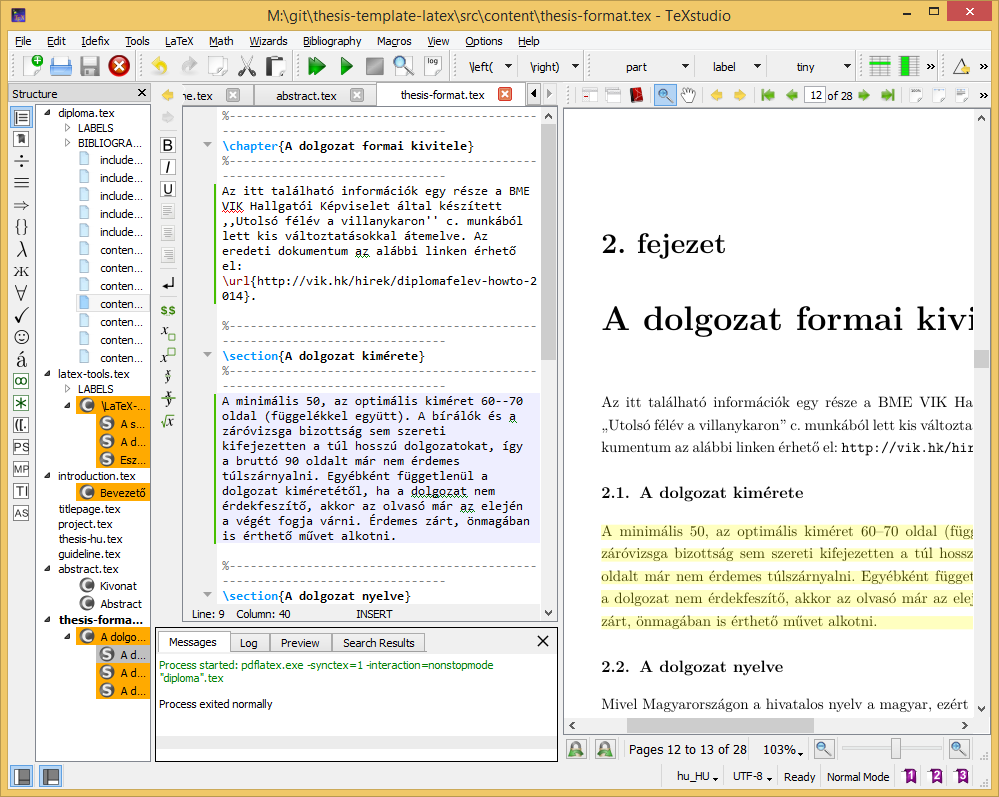
\includegraphics[width=67mm, keepaspectratio]{figures/TeXstudio.png}\hspace{1cm}
	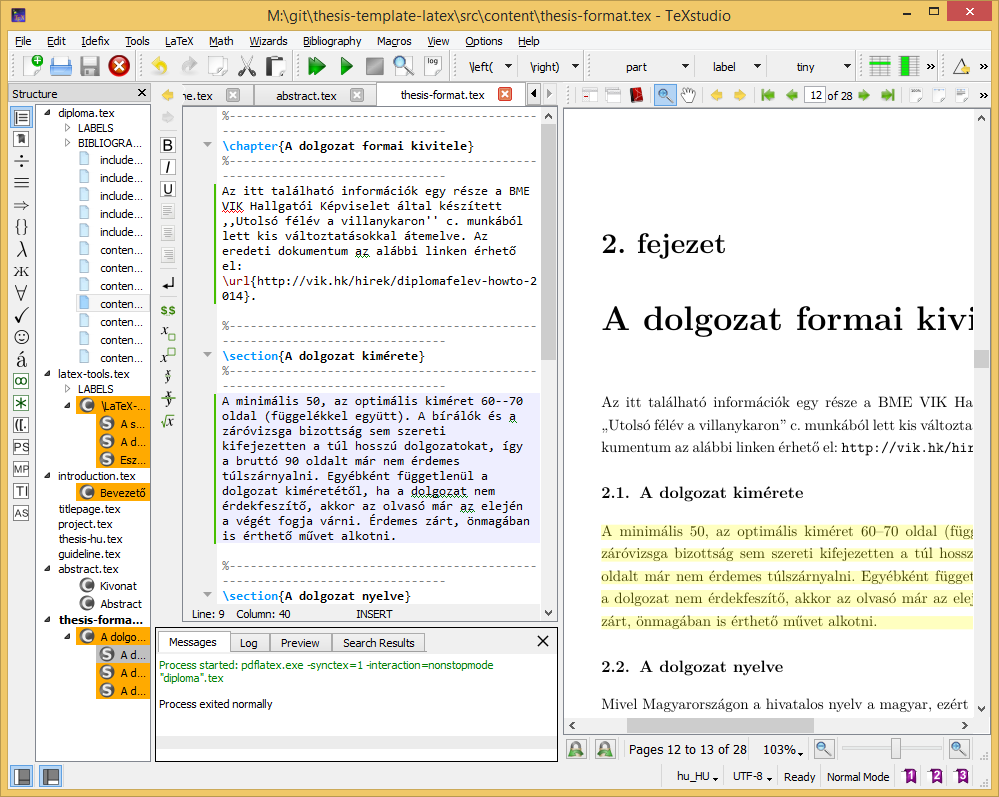
\includegraphics[width=67mm, keepaspectratio]{figures/TeXstudio.png}\\\vspace{5mm}
	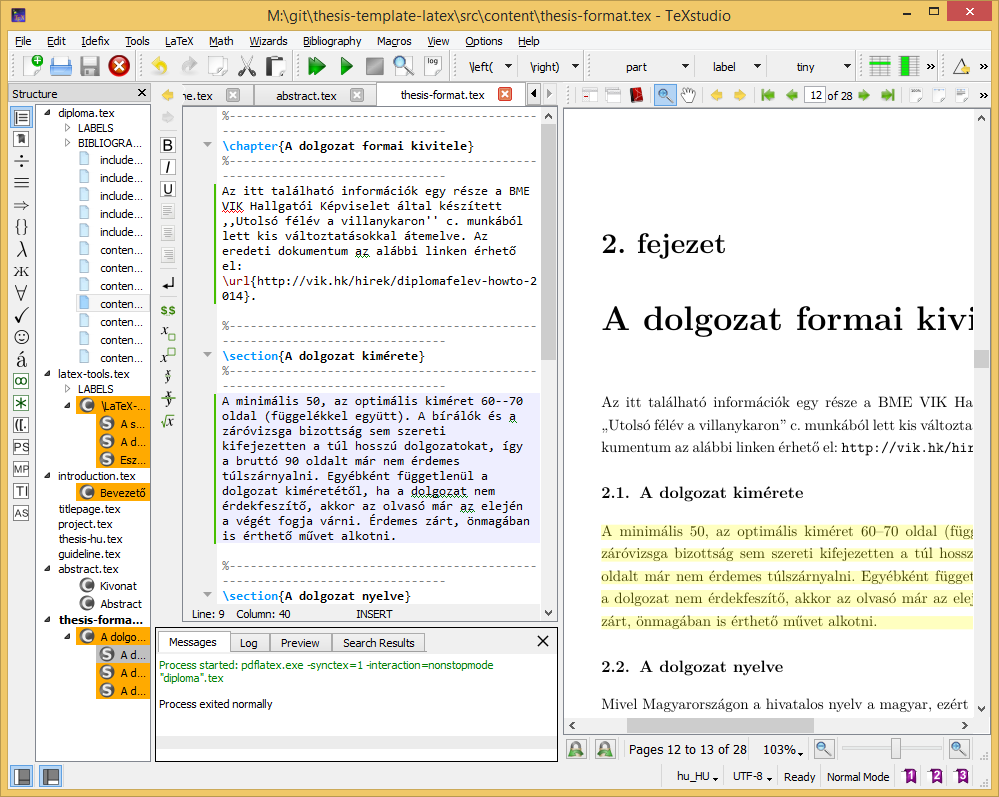
\includegraphics[width=67mm, keepaspectratio]{figures/TeXstudio.png}\hspace{1cm}
	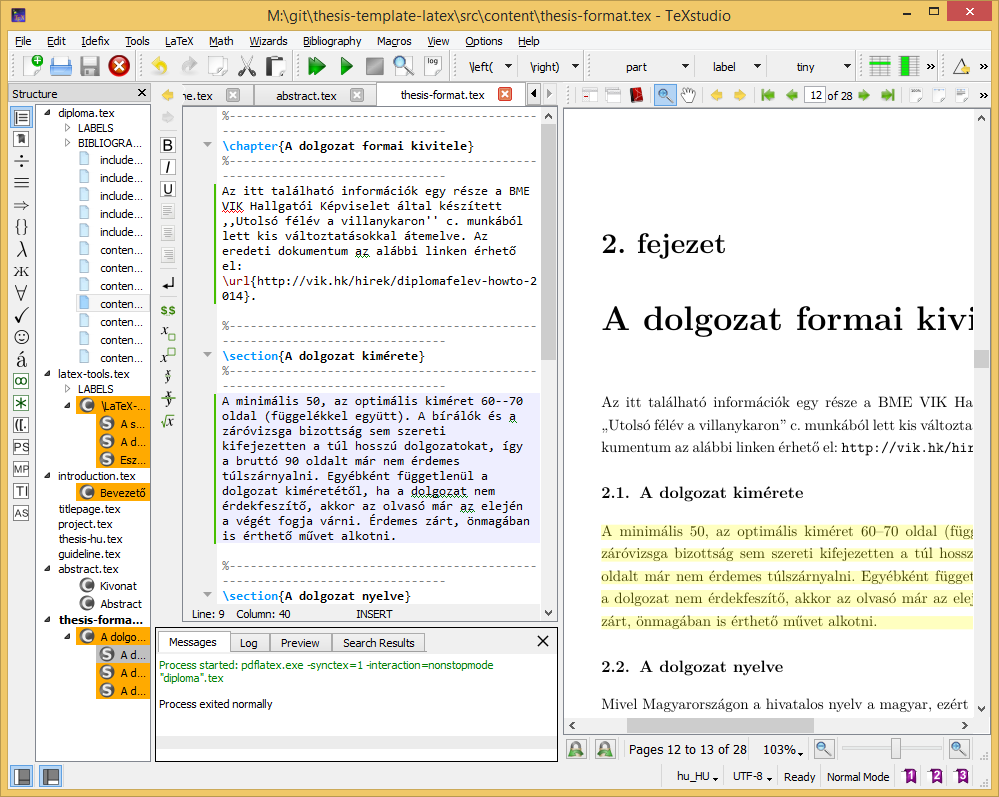
\includegraphics[width=67mm, keepaspectratio]{figures/TeXstudio.png}
	\caption{Több képfájl beillesztése esetén térközöket is érdemes használni.}
	\label{fig:HVSpaces}
\end{figure}

A táblázatok használatára \aref{tab:TabularExample}~táblázat mutat példát. A táblázatok formázásához hasznos tanácsokat találunk a \verb+booktabs+ csomag dokumentációjában.

\begin{table}[ht]
	\footnotesize
	\centering
	\begin{tabular}{ l c c }
		\toprule
		Órajel & Frekvencia & Cél pin \\
		\midrule
		CLKA & 100 MHz & FPGA CLK0\\
		CLKB & 48 MHz  & FPGA CLK1\\
		CLKC & 20 MHz  & Processzor\\
		CLKD & 25 MHz  & Ethernet chip \\
		CLKE & 72 MHz  & FPGA CLK2\\
		XBUF & 20 MHz  & FPGA CLK3\\
		\bottomrule
	\end{tabular}
	\caption{Az órajel-generátor chip órajel-kimenetei.}
	\label{tab:TabularExample}
\end{table}


%----------------------------------------------------------------------------
\section{Felsorolások és listák}
%----------------------------------------------------------------------------
Számozatlan felsorolásra mutat példát a jelenlegi bekezdés:
\begin{itemize}
	\item \emph{első bajusz:} ide lehetne írni az első elem kifejését,
	\item \emph{második bajusz:} ide lehetne írni a második elem kifejését,
	\item \emph{ez meg egy szakáll:} ide lehetne írni a harmadik elem kifejését.
\end{itemize}

Számozott felsorolást is készíthetünk az alábbi módon:
\begin{enumerate}
	\item \emph{első bajusz:} ide lehetne írni az első elem kifejését, és ez a kifejtés így néz ki, ha több sorosra sikeredik,
	\item \emph{második bajusz:} ide lehetne írni a második elem kifejését,
	\item \emph{ez meg egy szakáll:} ide lehetne írni a harmadik elem kifejését.
\end{enumerate}
A felsorolásokban sorok végén vessző, az utolsó sor végén pedig pont a szokásos írásjel. Ez alól kivételt képezhet, ha az egyes elemek több teljes mondatot tartalmaznak.

Listákban a dolgozat szövegétől elkülönítendő kódrészleteket, programsorokat, pszeudo-kódokat jeleníthetünk meg (\ref{lst:Example}.~kódrészlet).
\begin{lstlisting}[caption=A fenti számozott felsorolás \LaTeX-forráskódja,label=lst:Example]
\begin{enumerate}
	\item \emph{els(*@ő@*) bajusz:} ide lehetne írni az els(*@ő@*) elem kifejését,
	és ez a kifejtés így néz ki, ha több sorosra sikeredik,
	\item \emph{második bajusz:} ide lehetne írni a második elem kifejését,
	\item \emph{ez meg egy szakáll:} ide lehetne írni a harmadik elem kifejését.
\end{enumerate}
\end{lstlisting}
A lista keretét, háttérszínét, egész stílusát megválaszthatjuk. Ráadásul különféle programnyelveket és a nyelveken belül kulcsszavakat is definiálhatunk, ha szükséges. Erről bővebbet a \verb+listings+ csomag hivatalos leírásában találhatunk.

%----------------------------------------------------------------------------
\section{Képletek}
%----------------------------------------------------------------------------
Ha egy formula nem túlságosan hosszú, és nem akarjuk hivatkozni a szövegből, mint például a $e^{i\pi}+1=0$ képlet, \emph{szövegközi képletként} szokás leírni. Csak, hogy másik példát is lássunk, az $U_i=-d\Phi/dt$ Faraday-törvény a $\rot E=-\frac{dB}{dt}$ differenciális alakban adott Maxwell-egyenlet felületre vett integráljából vezethető le. Látható, hogy a \LaTeX-fordító a sorközöket betartja, így a szöveg szedése esztétikus marad szövegközi képletek használata esetén is.

Képletek esetén az általános konvenció, hogy a kisbetűk skalárt, a kis félkövér betűk ($\mathbf{v}$) oszlopvektort -- és ennek megfelelően $\mathbf{v}^T$ sorvektort -- a kapitális félkövér betűk ($\mathbf{V}$) mátrixot jelölnek. Ha ettől el szeretnénk térni, akkor az alkalmazni kívánt jelölésmódot célszerű külön alfejezetben definiálni. Ennek megfelelően, amennyiben $\mathbf{y}$ jelöli a mérések vektorát, $\mathbf{\vartheta}$ a paraméterek vektorát és $\hat{\mathbf{y}}=\mathbf{X}\vartheta$ a paraméterekben lineáris modellt, akkor a \emph{Least-Squares} értelemben optimális paraméterbecslő $\hat{\mathbf{\vartheta}}_{LS}=(\mathbf{X}^T\mathbf{X})^{-1}\mathbf{X}^T\mathbf{y}$ lesz.

Emellett kiemelt, sorszámozott képleteket is megadhatunk, ennél az \verb+equation+ és a \verb+eqnarray+ környezetek helyett a korszerűbb \verb+align+ környezet alkalmazását javasoljuk (több okból, különféle problémák elkerülése végett, amelyekre most nem térünk ki). Tehát
\begin{align}
\dot{\mathbf{x}}&=\mathbf{A}\mathbf{x}+\mathbf{B}\mathbf{u},\\
\mathbf{y}&=\mathbf{C}\mathbf{x},
\end{align}
ahol $\mathbf{x}$ az állapotvektor, $\mathbf{y}$ a mérések vektora és $\mathbf{A}$, $\mathbf{B}$ és $\mathbf{C}$ a rendszert leíró paramétermátrixok. Figyeljük meg, hogy a két egyenletben az egyenlőségjelek egymáshoz igazítva jelennek meg, mivel a mindkettőt az \& karakter előzi meg a kódban. Lehetőség van számozatlan kiemelt képlet használatára is, például
\begin{align}
\dot{\mathbf{x}}&=\mathbf{A}\mathbf{x}+\mathbf{B}\mathbf{u},\nonumber\\
\mathbf{y}&=\mathbf{C}\mathbf{x}\nonumber.
\end{align}
Mátrixok felírására az $\mathbf{A}\mathbf{x}=\mathbf{b}$ inhomogén lineáris egyenlet részletes kifejtésével mutatunk példát:
\begin{align}
\begin{bmatrix}
a_{11} & a_{12} & \dots & a_{1n}\\
a_{21} & a_{22} & \dots & a_{2n}\\
\vdots & \vdots & \ddots & \vdots\\
a_{m1} & a_{m2} & \dots & a_{mn}
\end{bmatrix}
\begin{pmatrix}x_1\\x_2\\\vdots\\x_n\end{pmatrix}=
\begin{pmatrix}b_1\\b_2\\\vdots\\b_m\end{pmatrix}.
\end{align}
A \verb+\frac+ utasítás hatékonyságát egy általános másodfokú tag átviteli függvényén keresztül mutatjuk be, azaz
\begin{align}
W(s)=\frac{A}{1+2T\xi s+s^2T^2}.
\end{align}
A matematikai mód minden szimbólumának és képességének a bemutatására természetesen itt nincs lehetőség, de gyors referenciaként hatékonyan használhatók a következő linkek:\\
\indent\url{http://www.artofproblemsolving.com/LaTeX/AoPS_L_GuideSym.php},\\
\indent\url{http://www.ctan.org/tex-archive/info/symbols/comprehensive/symbols-a4.pdf},\\
\indent\url{ftp://ftp.ams.org/pub/tex/doc/amsmath/short-math-guide.pdf}.\\
Ez pedig itt egy magyarázat, hogy miért érdemes \verb+align+ környezetet használni:\\
\indent\url{http://texblog.net/latex-archive/maths/eqnarray-align-environment/}.

%----------------------------------------------------------------------------
\section{Irodalmi hivatkozások}
\label{sec:HowtoReference}
%----------------------------------------------------------------------------
Egy \LaTeX~dokumentumban az irodalmi hivatkozások definíciójának két módja van. Az egyik a \verb+\thebibliograhy+ környezet használata a dokumentum végén, az \verb+\end{document}+ lezárás előtt.
\begin{lstlisting}
\begin{thebibliography}{9}

\bibitem{Lamport94} Leslie Lamport, \emph{\LaTeX: A Document Preparation System}.
Addison Wesley, Massachusetts, 2nd Edition, 1994.

\end{thebibliography}
\end{lstlisting}

Ezek után a dokumentumban a \verb+\cite{Lamport94}+ utasítással hivatkozhatunk a forrásra. A fenti megadás viszonylag kötetlen, a szerző maga formázza az irodalomjegyzéket (ami gyakran inkonzisztens eredményhez vezet).

Egy sokkal professzionálisabb módszer a BiB\TeX{} használata, ezért ez a sablon is ezt támogatja. Ebben az esetben egy külön szöveges adatbázisban definiáljuk a forrásmunkákat, és egy külön stílusfájl határozza meg az irodalomjegyzék kinézetét. Ez, összhangban azzal, hogy külön formátumkonvenció határozza meg a folyóirat-, a könyv-, a konferenciacikk- stb. hivatkozások kinézetét az irodalomjegyzékben (a sablon használata esetén ezzel nem is kell foglalkoznia a hallgatónak, de az eredményt célszerű ellenőrizni). felhasznált hivatkozások adatbázisa egy \verb+.bib+ kiterjesztésű szöveges fájl, amelynek szerkezetét a \Aref{lst:Bibtex} kódrészlet demonstrálja. A forrásmunkák bevitelekor a sor végi vesszők külön figyelmet igényelnek, mert hiányuk a BiB\TeX-fordító hibaüzenetét eredményezi. A forrásmunkákat típus szerinti kulcsszó vezeti be (\verb+@book+ könyv, \verb+@inproceedings+ konferenciakiadványban megjelent cikk, \verb+@article+ folyóiratban megjelent cikk, \verb+@techreport+ valamelyik egyetem gondozásában megjelent műszaki tanulmány, \verb+@manual+ műszaki dokumentáció esetén stb.). Nemcsak a megjelenés stílusa, de a kötelezően megadandó mezők is típusról-típusra változnak. Egy jól használható referencia a \url{http://en.wikipedia.org/wiki/BibTeX} oldalon található.

\begin{lstlisting}[caption=Példa szöveges irodalomjegyzék-adatbázisra Bib\TeX{} használata esetén.,label=lst:Bibtex]
@book{Wettl04,
  author    = {Ferenc Wettl and Gyula Mayer and Péter Szabó},
  publisher = {Panem Könyvkiadó},
  title     = {\LaTeX~kézikönyv},
  year      = {2004},
}

@article{Candy86,
  author       = {James C. Candy},
  journaltitle = {{IEEE} Trans.\ on Communications},
  month        = {01},
  note         = {\doi{10.1109/TCOM.1986.1096432}},
  number       = {1},
  pages        = {72--76},
  title        = {Decimation for Sigma Delta Modulation},
  volume       = {34},
  year         = {1986},
}

@inproceedings{Lee87,
  author    = {Wai L. Lee and Charles G. Sodini},
  booktitle = {Proc.\ of the IEEE International Symposium on Circuits and Systems},
  location  = {Philadelphia, PA, USA},
  month     = {05~4--7},
  pages     = {459--462},
  title     = {A Topology for Higher Order Interpolative Coders},
  vol       = {2},
  year      = {1987},
}

@thesis{KissPhD,
  author      = {Peter Kiss},
  institution = {Technical University of Timi\c{s}oara, Romania},
  month       = {04},
  title       = {Adaptive Digital Compensation of Analog Circuit Imperfections for Cascaded Delta-Sigma Analog-to-Digital Converters},
  type        = {phdthesis},
  year        = {2000},
}

@manual{Schreier00,
  author       = {Richard Schreier},
  month        = {01},
  note         = {\url{http://www.mathworks.com/matlabcentral/fileexchange/}},
  organization = {Oregon State University},
  title        = {The Delta-Sigma Toolbox v5.2},
  year         = {2000},
}

@misc{DipPortal,
  author       = {{Budapesti Műszaki és Gazdaságtudományi Egyetem Villamosmérnöki és Informatikai Kar}},
  howpublished = {\url{http://diplomaterv.vik.bme.hu/}},
  title        = {Diplomaterv portál (2011. február 26.)},
}

@incollection{Mkrtychev:1997,
  author    = {Mkrtychev, Alexey},
  booktitle = {Logical Foundations of Computer Science},
  doi       = {10.1007/3-540-63045-7_27},
  editor    = {Adian, Sergei and Nerode, Anil},
  isbn      = {978-3-540-63045-6},
  pages     = {266-275},
  publisher = {Springer Berlin Heidelberg},
  series    = {Lecture Notes in Computer Science},
  title     = {Models for the logic of proofs},
  url       = {http://dx.doi.org/10.1007/3-540-63045-7_27},
  volume    = {1234},
  year      = {1997},
}
\end{lstlisting}

A stílusfájl egy \verb+.sty+ kiterjesztésű fájl, de ezzel lényegében nem kell foglalkozni, mert vannak beépített stílusok, amelyek jól használhatók. Ez a sablon a BiB\TeX-et használja, a hozzá tartozó adatbázisfájl a \verb+mybib.bib+ fájl. Megfigyelhető, hogy az irodalomjegyzéket a dokumentum végére (a \verb+\end{document}+ utasítás elé) beillesztett \verb+\bibliography{mybib}+ utasítással hozhatjuk létre, a stílusát pedig ugyanitt a  \verb+\bibliographystyle{plain}+ utasítással adhatjuk meg. Ebben az esetben a \verb+plain+ előre definiált stílust használjuk (a sablonban is ezt állítottuk be). A \verb+plain+ stíluson kívül természetesen számtalan más előre definiált stílus is létezik. Mivel a \verb+.bib+ adatbázisban ezeket megadtuk, a BiB\TeX-fordító is meg tudja különböztetni a szerzőt a címtől és a kiadótól, és ez alapján automatikusan generálódik az irodalomjegyzék a stílusfájl által meghatározott stílusban.

Az egyes forrásmunkákra a szövegből továbbra is a \verb+\cite+ paranccsal tudunk hivatkozni, így \aref{lst:Bibtex}.~kódrészlet esetén a hivatkozások rendre \verb+\cite{Wettl04}+, \verb+\cite{Candy86}+, \verb+\cite{Lee87}+, \verb+\cite{KissPhD}+, \verb+\cite{Schreirer00}+,
\verb+\cite{Mkrtychev:1997}+ és \verb+\cite{DipPortal}+. Az egyes forrásmunkák sorszáma az irodalomjegyzék bővítésekor változhat. Amennyiben az aktuális számhoz illeszkedő névelőt szeretnénk használni, használjuk az \verb+\acite{}+ parancsot.

Az irodalomjegyzékben alapértelmezésben csak azok a forrásmunkák jelennek meg, amelyekre található hivatkozás a szövegben, és ez így alapvetően helyes is, hiszen olyan forrásmunkákat nem illik az irodalomjegyzékbe írni, amelyekre nincs hivatkozás.

Mivel a fordítási folyamat során több lépésben oldódnak fel a szimbólumok, ezért gyakran többször is le kell fordítani a dokumentumot. Ilyenkor ez első 1-2 fordítás esetleg szimbólum-feloldásra vonatkozó figyelmeztető üzenettel zárul. Ha hibaüzenettel zárul bármelyik fordítás, akkor nincs értelme megismételni, hanem a hibát kell megkeresni. A \verb+.bib+ fájl megváltoztatáskor sokszor nincs hatása a változtatásnak azonnal, mivel nem mindig fut újra a BibTeX fordító. Ezért célszerű a változtatás után azt manuálisan is lefuttatni (TeXstudio esetén \verb+Tools/Bibliography+).

Hogy a szövegbe ágyazott hivatkozások kinézetét demonstráljuk, itt most sorban meghivatkozzuk a \cite{Wettl04}, \cite{Candy86}, \cite{Lee87}, \cite{KissPhD}, \cite{Schreier00} és \acite{Mkrtychev:1997}\footnote{Informatikai témában gyakran hivatkozunk cikkeket a Springer LNCS valamely kötetéből, ez a hivatkozás erre mutat egy helyes példát.} forrásmunkát, valamint \acite{DipPortal} weboldalt.

Megjegyzendő, hogy az ékezetes magyar betűket is tartalmazó \verb+.bib+ fájl az \verb+inputenc+ csomaggal betöltött \verb+latin2+ betűkészlet miatt fordítható. Ugyanez a \verb+.bib+ fájl hibaüzenettel fordul egy olyan dokumentumban, ami nem tartalmazza a \verb+\usepackage[latin2]{inputenc}+ sort. Speciális igény esetén az irodalmi adatbázis általánosabb érvényűvé tehető, ha az ékezetes betűket speciális latex karakterekkel helyettesítjük a \verb+.bib+ fájlban, pl. á helyett \verb+\'{a}+-t vagy ő helyett \verb+\H{o}+-t írunk.

Oldaltörés következik (ld. forrás).
\newpage

%----------------------------------------------------------------------------
\section{A dolgozat szerkezete és a forrásfájlok}
%----------------------------------------------------------------------------
A diplomatervsablonban a TeX fájlok két alkönyvtárban helyezkednek el. Az \verb+include+ könyvtárban azok szerepelnek, amiket tipikusan nem kell szerkesztenünk, ezek a sablon részei (pl. címoldal). A \verb+content+ alkönyvtárban pedig a saját munkánkat helyezhetjük el. Itt érdemes az egyes fejezeteket külön \TeX{} állományokba rakni.

A diplomatervsablon (a kari irányelvek szerint) az alábbi fő fejezetekből áll:
\begin{enumerate}
	\item 1 oldalas \emph{tájékoztató} a szakdolgozat/diplomaterv szerkezetéről (\verb+include/guideline.tex+), ami a végső dolgozatból törlendő,
	\item \emph{feladatkiírás} (\verb+include/project.tex+), a dolgozat nyomtatott verzójában ennek a helyére kerül a tanszék által kiadott, a tanszékvezető által aláírt feladatkiírás, a dolgozat elektronikus verziójába pedig a feladatkiírás egyáltalán ne kerüljön bele, azt külön tölti fel a tanszék a diplomaterv-honlapra,
	\item \emph{címoldal} (\verb+include/titlepage.tex+),
	\item \emph{tartalomjegyzék} (\verb+thesis.tex+),
	\item a diplomatervező \emph{nyilatkozat}a az önálló munkáról (\verb+include/declaration.tex+),
	\item 1-2 oldalas tartalmi \emph{összefoglaló} magyarul és angolul, illetve elkészíthető még további nyelveken is (\verb+content/abstract.tex+),
	\item \emph{bevezetés}: a feladat értelmezése, a tervezés célja, a feladat indokoltsága, a diplomaterv felépítésének rövid összefoglalása (\verb+content/introduction.tex+),
	\item sorszámmal ellátott \emph{fejezetek}: a feladatkiírás pontosítása és részletes elemzése, előzmények (irodalomkutatás, hasonló alkotások), az ezekből levonható következtetések, a tervezés részletes leírása, a döntési lehetőségek értékelése és a választott megoldások indoklása, a megtervezett műszaki alkotás értékelése, kritikai elemzése, továbbfejlesztési lehetőségek,
	\item esetleges \emph{köszönetnyilvánítás}ok (\verb+content/acknowledgement.tex+),
	\item részletes és pontos \emph{irodalomjegyzék} (ez a sablon esetében automatikusan generálódik a \verb+thesis.tex+ fájlban elhelyezett \verb+\bibliography+ utasítás hatására, \az+\refstruc{sec:HowtoReference}ban leírtak szerint),
	\item \emph{függelékek} (\verb+content/appendices.tex+).
\end{enumerate}

A sablonban a fejezetek a \verb+thesis.tex+ fájlba vannak beillesztve \verb+\include+ utasítások segítségével. Lehetőség van arra, hogy csak az éppen szerkesztés alatt álló \verb+.tex+ fájlt fordítsuk le, ezzel lerövidítve a fordítási folyamatot. Ezt a lehetőséget az alábbi kódrészlet biztosítja a \verb+thesis.tex+ fájlban.
\begin{lstlisting}
\includeonly{
	guideline,%
	project,%
	titlepage,%
	declaration,%
	abstract,%
	introduction,%
	chapter1,%
	chapter2,%
	chapter3,%
	acknowledgement,%
	appendices,%
}
\end{lstlisting}

Ha az alábbi kódrészletben az egyes sorokat a \verb+%+ szimbólummal kikommentezzük, akkor a megfelelő \verb+.tex+ fájl nem fordul le. Az oldalszámok és a tartalomjegyék természetesen csak akkor billennek helyre, ha a teljes dokumentumot lefordítjuk.

%----------------------------------------------------------------------------
\newpage
\section{Alapadatok megadása}
%----------------------------------------------------------------------------
A diplomaterv alapadatait (cím, szerző, konzulens, konzulens titulusa) a \verb+thesis.tex+ fájlban lehet megadni.

%----------------------------------------------------------------------------
\section{Új fejezet írása}
%----------------------------------------------------------------------------
A főfejezetek külön \verb+content+ könyvtárban foglalnak helyet. A sablonhoz 3 fejezet készült. További főfejezeteket úgy hozhatunk létre, ha új \TeX~fájlt készítünk a fejezet számára, és a \verb+thesis.tex+ fájlban, a \verb+\include+ és \verb+\includeonly+ utasítások argumentumába felvesszük az új \verb+.tex+ fájl nevét.


%----------------------------------------------------------------------------
\section{Definíciók, tételek, példák}
%----------------------------------------------------------------------------

\begin{definition}[Fluxuskondenzátor térerőssége]
Lorem ipsum dolor sit amet, consectetur adipiscing elit, sed do eiusmod tempor incididunt ut labore et dolore magna aliqua. Ut enim ad minim veniam, quis nostrud exercitation ullamco laboris nisi ut aliquip ex ea commodo consequat.
\end{definition}

\begin{example}
Példa egy példára. Duis aute irure dolor in reprehenderit in voluptate velit esse cillum dolore eu fugiat nulla pariatur. Excepteur sint occaecat cupidatat non proident, sunt in culpa qui officia deserunt mollit anim id est laborum.
\end{example}

\begin{theorem}[Kovács tétele]
Duis aute irure dolor in reprehenderit in voluptate velit esse cillum dolore eu fugiat nulla pariatur. Excepteur sint occaecat cupidatat non proident, sunt in culpa qui officia deserunt mollit anim id est laborum.
\end{theorem}



% Acknowledgements
%~~~~~~~~~~~~~~~~~~~~~~~~~~~~~~~~~~~~~~~~~~~~~~~~~~~~~~~~~~~~~~~~~~~~~~~~~~~~~~~~~~~~~~
%%----------------------------------------------------------------------------
\chapter*{\koszonetnyilvanitas}\addcontentsline{toc}{chapter}{\koszonetnyilvanitas}
%----------------------------------------------------------------------------

Köszönöm munkatársaimnak a szakdolgozat megírásával kapcsolatos szakmai segítséget, valamint a hatékony munkához szükséges környezetet. Külön köszönettel tartozom továbbá konzulensemnek, dr. Czap Lászlónak, az egész éves feladat során nyújtott segítségért és jó tanácsokért.


% List of Figures, Tables
%~~~~~~~~~~~~~~~~~~~~~~~~~~~~~~~~~~~~~~~~~~~~~~~~~~~~~~~~~~~~~~~~~~~~~~~~~~~~~~~~~~~~~~
%\listoffigures\addcontentsline{toc}{chapter}{\abrakjegyzeke}
%\listoftables\addcontentsline{toc}{chapter}{\tablazatokjegyzeke}


% Bibliography
%~~~~~~~~~~~~~~~~~~~~~~~~~~~~~~~~~~~~~~~~~~~~~~~~~~~~~~~~~~~~~~~~~~~~~~~~~~~~~~~~~~~~~~
%\bibliography{bib/mybib}
\addcontentsline{toc}{chapter}{\irodalomjegyzek}


% Appendix
%~~~~~~~~~~~~~~~~~~~~~~~~~~~~~~~~~~~~~~~~~~~~~~~~~~~~~~~~~~~~~~~~~~~~~~~~~~~~~~~~~~~~~~
%%----------------------------------------------------------------------------
\appendix
%----------------------------------------------------------------------------
\chapter*{\fuggelek}\addcontentsline{toc}{chapter}{\fuggelek}
\setcounter{chapter}{\appendixnumber}
%\setcounter{equation}{0} % a fofejezet-szamlalo az angol ABC 6. betuje (F) lesz
\numberwithin{equation}{section}
\numberwithin{figure}{section}
\numberwithin{lstlisting}{section}
%\numberwithin{tabular}{section}

\appendix

% Table generated by Excel2LaTeX from sheet 'All'
\begin{table}[htbp]
	\centering
	\small
	\caption{Add caption}
	\begin{tabular}{p{.20\linewidth}p{.80\linewidth}}
		Attribútum név & Attribútum funkciója \\
		A\_ACTIVITY\_INDEX & Activity számláló azonosítója, ha egy ciklusban szerepel \\
		A\_COMPLETED & Az activity befejezésének időpontja \\
		A\_DESCRIPTION & Maximum 300 karakteres, beszédes leírása az activity-nek \\
		A\_ID & Activity egyedi azonosítója \\
		A\_LASTMODIFIED & Az activity utolsó módosításának dátuma \\
		A\_LOCK\_COUNT & A függőben lévő feladatok az activity-n \\
		A\_LOOP\_COUNT & Iteráció specifikus érték. Az eltelt iterációk száma. \\
		A\_LOOP\_RUNCOUNT & Aszinkron ciklusos activity-k értéke. A hátralévő iterációk száma \\
		A\_NAME & Acvitiy beszédes neve. Segíti az activity azonosítását \\
		A\_PRIORITY & Activity prioritása. \\
		A\_PROCESS\_ID & Az adott activity-hez tartozó process egyedi azonosítója. Ezen keresztül köthető össze a process táblával \\
		A\_RESULT\_DETAIL & Végeredmény beszédes leírása \\
		A\_RESULT\_SUMMARY & Két karakteres leírása a végeredménynek. Ezzel a mezővel szűrhetünk az activity-k végeredményére. \\
		A\_RETRY\_COUNT & Próbálkozások száma az activity végrehajtására \\
		A\_SHORT\_DETAIL & Rövid, szöveges leírása az activity végeredményének \\
		A\_STARTED & Az activity indításának időpontja \\
		A\_STATE & Az activity aktuális állapota. Ezzel szűrhetünk pl a futó, a megállított, a befejezett, stb állapotokra. \\
		A\_SUBPROCESS\_ID & Az activity-hez kapcsolódó subprocess azonosítója. \\
		A\_SUBTYPE & Kézi activity-knél altípus, pl ezzel különböztethető meg a jóváhagyás/elutasítási, és az információ adási kérés. \\
		A\_TYPE & Az activity típusa, egy karakterként tárolva. Pl: kézi (M), alkalmazás (A), subprocess (S) \\
		P\_COMMENTS & Megjegyzések a process-hez \\
		P\_COMPLETED & A process befejezésének ideje. \\
		P\_DEFINITION\_ID & A process definíciójának azonosítója. \\
		P\_DESCRIPTION & Process szöveges leírása. \\
		P\_ID & Adott process azonosítója. \\
		P\_LASTMODIFIED & A process utolsó változásának időpontja. \\
		P\_NAME & A process neve. \\
		P\_NOTIFY & Megadja, hogy ki értesüljön a process befejeztekor. \\
		P\_PARENT\_ACTIVITY\_ID & Az adott processhez tartozó szülő activity azonosítója, ha van neki. \\
		P\_PARENT\_ID & A szülő process azonosítója, ha van neki. \\
		P\_PRIORITY & A process prioritása. \\
		P\_REQUESTEE & Annak a DN-je, aki számára a process végrehajtásra kerül. \\
		P\_REQUESTEE\_NAME & Annak a neve, aki számára a process végrehajtásra kerül. \\
		P\_REQUESTER & A process kérelmezőjének a DN-je. \\
		P\_REQUESTER\_NAME & A process kérelmezőjének a neve. \\
		P\_REQUESTER\_TYPE & A process kérelmezőjének a típusa. Pl végfelhasználó (U), ISIM System (P), Workflow (S). \\
		P\_RESULT\_DETAIL & Részletes információk a process eredményéről. \\
		P\_RESULT\_SUMMARY & A process végeredménye, két karakterként reprezentálva. Pl: jóváhagyva (AA), elutasítva (AR), sikertelen(SF). \\
		P\_ROOT\_PROCESS\_ID & A legmagasabb szinten álló szülő process azonosítója. \\
		P\_SCHEDULED & A process ütemezett indítási időpontja. \\
		P\_SHORT\_DETAIL & Rövid összefoglaló a process eredményéről. \\
		P\_STARTED & A process indításának ideje. \\
		P\_STATE & A process aktuális állapota. Pl: futó (R), kész (C), megállított (A) \\
		P\_SUBJECT & A process alanya. \\
		P\_SUBJECT\_ACCESS\_ID & A kérelmezett hozzáférés DN-je. (Ha a process hozzáférési kérelem volt) \\
		P\_SUBJECT\_ACCESS\_NAME & A kérelmezett hozzáférés neve. (Ha a process hozzáférési kérelem volt) \\
		P\_SUBJECT\_PROFILE & Az alany LDAP szintű típusa. \\
		P\_SUBJECT\_SERVICE & Az a service, amihez az alany tartozik. \\
		P\_SUBMITTED & A process létrehozásának időpontja. \\
		P\_TENANT & A kérelmezőhöz tartozó tartomány DN-je. \\
		P\_TYPE & 2 karakteres kódja a process típusának. Pl: új felhasználó (UA), jelszóváltoztatás (AP). \\
		PL\_ACTIVITY\_ID & A processlog eseményhez tartozó activity azonosítója. \\
		PL\_CREATED & A processlog esemény létrehozásának ideje. \\
		PL\_DATA\_ID & Az adat azonosítója adat változás esetén. \\
		PL\_EVENTTYPE & Az adott log esemény típus kódja. Pl: activity létrehozva (AC), activity állapot változott (AS) \\
		PL\_ID & Az adott process log esemény azonosítója. \\
		PL\_NEW\_DATA & Új adatok az adatváltozási esemény során, ha azok mérete nagyobb mint egy limit. \\
		PL\_NEW\_PARTICIPANT\_ID & Az új résztvevő azonosítója feladat delegáció esetén. \\
		PL\_NEW\_PARTICIPANT\_TYPE & Az új résztvevő típusa feladat delegáció esetén. \\
		PL\_NEW\_STATE & Új típus, egy típus változási esemény során. \\
		PL\_OLD\_PARTICIPANT\_ID & Feladat delegációs esemény esetén a régi résztvevő azonosítója. \\
		PL\_OLD\_PARTICIPANT\_TYPE & Feladat delegációs esemény esetén a régi résztvevő típusa. \\
		PL\_OLD\_STATE & Régi típus egy típus változási esemény során. \\
		PL\_PROCESS\_ID & A process azonosítója, amihez a process log esemény tartozik. \\
		PL\_REQUESTOR & Igénylő neve felhasználókkal kapcsolatos eseményeknél \\
		PL\_REQUESTOR\_DN & Igénylő DN-je felhasználókkal kapcsolatos eseményeknél \\
		PL\_REQUESTOR\_TYPE & Igénylő típusa felhasználókkal kapcsolatos eseményeknél \\
		PL\_SMALL\_NEW\_DATA & Új adatok az adatváltozási esemény során, ha azok mérete kisebb mind egy limit. \\
	\end{tabular}%
	\label{tab:allprops}%
\end{table}%

%----------------------------------------------------------------------------
\clearpage\section{Válasz az ,,Élet, a világmindenség, meg minden'' kérdésére}
%----------------------------------------------------------------------------
A Pitagorasz-tételből levezetve
\begin{align}
c^2=a^2+b^2=42.
\end{align}
A Faraday-indukciós törvényből levezetve
\begin{align}
\rot E=-\frac{dB}{dt}\hspace{1cm}\longrightarrow \hspace{1cm}
U_i=\oint\limits_\mathbf{L}{\mathbf{E}\mathbf{dl}}=-\frac{d}{dt}\int\limits_A{\mathbf{B}\mathbf{da}}=42.
\end{align}


%\label{page:last}
\end{document}
